\chapter{\texorpdfstring{$p$}{p}- to \texorpdfstring{$s$}{s}-wave phase transition} % Main chapter title

\label{Chapter6} 
\fancyhead[LO, RE]{Part II. \emph{Kitaev wires}}
\chead{Chapter 6. \emph{\texorpdfstring{$p$}{p}- to \texorpdfstring{$s$}{s}-wave phase transition}} % This is for the header on each page - perhaps a shortened title

%----------------------------------------------------------------------------------------
The previous chapter gives a rather abstract discussion of the topological properties of the double wire system. In this chapter we return to a concrete calculation of the pairing potentials by solving the BCS equations self-consistently, contrary to the approach found in much of the literature on the subject. The price for this more ambitious approach is that we use mean field theory. In section \ref{sec.assumptions} we briefly summarize the assumptions made so far. In section \ref{sec.2wiresCrossover_energy} we compute the ground state energy and find the energetically favourable transition. In section \ref{sec.pairingsfunctionalbehaviour} we study the functional behaviour of the pairings for the energetically favourable transition. Here we verify that the pairings are in fact $p$- and $s$-wave types. In section \ref{sec.pairwavefunctions} we study the pair wave functions. In section \ref{sec.2wires_crossover_control_coherence_length} we characterize the effective interactions and study how one can use the coherence length to control the $p$- to $s$-wave phase transition. This results in a phase diagram as a function of the interwire distance and the coherence length. Finally, in section \ref{sec.physicaldiscrepancies} we briefly discuss the results, physical discrepancies and possible improvements within mean field theory.

\section{Assumptions} \label{sec.assumptions}
Before performing the numerical calculation, it is worthwhile to summarize what assumptions, we have made so far. 

\begin{table}[htb]
\def\arraystretch{1.5}
\centering
\begin{tabular}{|l|l|r|l|}
		\hline \textbf{Quantity} 		& \textbf{Parameters} 					& \textbf{Assumption}								& \textbf{Reason}	\\ \hline
		\hline Transverse energy gap 	& $\omega_t = \frac{1}{\sqrt{m_Fl_t}}$ 	& $(k_Fl_t)^2 	 	\ll 1$ 							& Trap in transverse ground state \\
		\hline Trapping width 		 	& $l_t, d$ 								& $l_t / d 	\ll 1$ 									& Distinguishable wires \\
		\hline $B-B$ scattering length 	& $g_B = \frac{4\pi a_B}{m_B}$			& $(n_Ba_B^3)^{1/3}	\ll 1$							& Negligible BEC depletion  \\
		\hline $\omega_n = 0$ limit  	& $v_F,c_0$								& $v_F/c_0 \ll 1$ 									& Negligible retardation effects  \\
		\hline $B-F$ scattering length 	& $a_{BF}, n_B, n_F$ 					& \def\arraystretch{1.2} \begin{tabular}{@{}r@{}} $(n_Ba_{BF}^3)^{1/3} \ll 1$ \\ $n_Fa_{BF} \ll 1$ \end{tabular}	&\def\arraystretch{1.2}\begin{tabular}{@{}l@{}}$2^{\text{nd}}$ order perturbation theory \\ for induced interaction \end{tabular} \\
		\hline 
\end{tabular}
\caption{Summary of the assumptions made so far. $m_r = \frac{m_Fm_B}{m_F + m_B}$ is the reduced mass. B and F refer to Bosons and Fermions respectively. $\omega_n$ is the bosonic Matsubara frequencies associated with the induced interaction.}
\label{tab.assumptions}
\end{table} 

To trap the fermions in one dimension we assumed that the transverse energy, $\omega_t$, is much larger than the Fermi energy, $\epsilon_{F,0}$. This lead to the requirement in the first line of table \ref{tab.assumptions}, with $l_t$ the wire width. To have distinguishable wires we assumed that the wire width is much smaller than the interwire distance, $l_t / d \ll 1$. This is line two of the table. To have neglible ground state depletion of the condensate, we saw in equation \eqref{eq.excitedbosonsBEC} that we needed to assume $(n_Ba_B^3)^{1/3}\ll 1$. This is line three of the table. Further, to be able to neglect retardation effects, we needed to assume that the fermions moves slowly relative to the quasiparticles in the BEC. This is line four in the table. Finally, to ensure that we only need to work to second order in the Bose-Fermi interaction strength $g_{BF}$ when calculating the induced interaction, we need $(n_Ba_{BF}^3)^{1/3} \ll 1$ and $n_Fa_{BF} \ll 1$. This is line five of the table. 


\section{Self-consistent solution to the BCS equations}
\label{sec.2wiresCrossover_energy}
In this section we numerically calculate the pairing potentials self-consistently. We show that the energetically favourable transition exhibits a coexistence of the intra- and interwire pairings. The coexistence is such that it breaks the $T^2 = -\mathbb{I}$ symmetry and the edge states become gradually gapped. 

We first come with an energy analysis as described after equation \eqref{eq.2wiresGrandGroundStateEnergy}. First, for a particular value of the interwire distance, $d$, we come with an initial guess for the pairing and the chemical potentials. Second, we insert this initial guess into the gap equations \eqref{eq.2wiresgapequations} and an updated version of the pairings is obtained. Third, this is inserted into the number equation \eqref{eq.2wiresnumberequation}, where the chemical potential is varied until the number equation is fulfilled. Finally, this is iterated until the pairings are not altered by more than $0.1$\textperthousand. For each step of $d$ we then return to the same initial guess for the pairings to avoid any hysteresis in the analysis. We then use equation \eqref{eq.2wiresGrandGroundStateEnergy} to calculate the grand potential, $\Phi$, and in turn the energy $E_0 = \Phi + 2\mu N_F$. The pairings at the Fermi momentum, $|\Delta^{11}_{k_F}|$ and $|\Delta^{12}_{k_F}|$, are also recorded. 

It is possible to come with some rather well-educated initial guesses for the pairing and the chemical potentials. We expect that the chemical potential is not altered significantly from the one for the free gas, and so $\mu(T = 0)/\epsilon_{F,0} = 1$ is a good initial guess. The \textit{intra}wire pairing is odd in $k$ and inspecting the gap equation, there are only significant contributions around $k' = k$. Hence, we expect that the pairing goes to 0 for large values of $k/k_F$. Similarly, the \textit{inter}wire pairing is even in $k$ and also goes to zero for large $k / k_F$. 

The analysis is performed in four cases for the following set of parameters: the Bose gas parameter is set to $(n_Ba_B^3)^{1/3} = 0.01$. The Bose-Fermi gas parameter is set to $(n_Ba_{BF}^3)^{1/3} = 0.1$. The wire width is set to $l_t = 0$. The ratio of the boson and fermion masses is $m_B / m_F = 7/40$ and the relative interparticle distance is $n_F / n_B^{1/3} = 0.215$. This set of parameters means that the Fermi speed, $v_F$, relative to the speed of the phonons in the BEC, $c_0$, is: $v_F/c_0 = 0.33$. Hence, the assumptions of table \ref{tab.assumptions} are met. The ratio of masses, $m_B / m_F = 7 / 40$, corresponds to a mixture of bosonic $^{7}\text{Li}$ and fermionic $^{40}\text{K}$. The used parameters are in this sense experimentally relevant.   

\subsection{\texorpdfstring{$\Delta^{12} = 0$ or $\Delta^{11} = 0$}{Zero inter- or intrawire pairing}}
In this subsection we cover the first two cases. First, we let $\Delta^{12} = 0$ and search for nonzero $\Delta^{11}$. This results in the dashed curve in figure \ref{fig.2wiresE0ddepend} for the specified set of parameters. Hence, this describes the situation where we only have intrawire pairing. It is independent of the interwire distance, $d$. Conversely, we can let $\Delta^{11} = 0 = \Delta^{22}$ and search for nonzero $\Delta^{12}$. This results in the dash-dotted curve. Since the interwire interaction decreases with increasing interwire distances, $d$, the energy associated with a resulting interwire pairing must increase monotonically with $d$. This is also observed. The two curves thus intersect at some critical distance, $d_c$. In the present case $k_Fd_c \approx 0.759$. The naively expected behaviour is then the following. For large interwire distances, $d$, the intrawire pairing is energetically favourable and is therefore the only one present. As we decrease $d$ we get to the critical distance, $d_c$, where the interwire pairing becomes favourable instead. For $d < d_c$ we would then expect the interwire pairing to be the only one present. 

\begin{figure} 
\begin{center}  
% GNUPLOT: LaTeX picture with Postscript
\begingroup
  \makeatletter
  \providecommand\color[2][]{%
    \GenericError{(gnuplot) \space\space\space\@spaces}{%
      Package color not loaded in conjunction with
      terminal option `colourtext'%
    }{See the gnuplot documentation for explanation.%
    }{Either use 'blacktext' in gnuplot or load the package
      color.sty in LaTeX.}%
    \renewcommand\color[2][]{}%
  }%
  \providecommand\includegraphics[2][]{%
    \GenericError{(gnuplot) \space\space\space\@spaces}{%
      Package graphicx or graphics not loaded%
    }{See the gnuplot documentation for explanation.%
    }{The gnuplot epslatex terminal needs graphicx.sty or graphics.sty.}%
    \renewcommand\includegraphics[2][]{}%
  }%
  \providecommand\rotatebox[2]{#2}%
  \@ifundefined{ifGPcolor}{%
    \newif\ifGPcolor
    \GPcolorfalse
  }{}%
  \@ifundefined{ifGPblacktext}{%
    \newif\ifGPblacktext
    \GPblacktexttrue
  }{}%
  % define a \g@addto@macro without @ in the name:
  \let\gplgaddtomacro\g@addto@macro
  % define empty templates for all commands taking text:
  \gdef\gplbacktext{}%
  \gdef\gplfronttext{}%
  \makeatother
  \ifGPblacktext
    % no textcolor at all
    \def\colorrgb#1{}%
    \def\colorgray#1{}%
  \else
    % gray or color?
    \ifGPcolor
      \def\colorrgb#1{\color[rgb]{#1}}%
      \def\colorgray#1{\color[gray]{#1}}%
      \expandafter\def\csname LTw\endcsname{\color{white}}%
      \expandafter\def\csname LTb\endcsname{\color{black}}%
      \expandafter\def\csname LTa\endcsname{\color{black}}%
      \expandafter\def\csname LT0\endcsname{\color[rgb]{1,0,0}}%
      \expandafter\def\csname LT1\endcsname{\color[rgb]{0,1,0}}%
      \expandafter\def\csname LT2\endcsname{\color[rgb]{0,0,1}}%
      \expandafter\def\csname LT3\endcsname{\color[rgb]{1,0,1}}%
      \expandafter\def\csname LT4\endcsname{\color[rgb]{0,1,1}}%
      \expandafter\def\csname LT5\endcsname{\color[rgb]{1,1,0}}%
      \expandafter\def\csname LT6\endcsname{\color[rgb]{0,0,0}}%
      \expandafter\def\csname LT7\endcsname{\color[rgb]{1,0.3,0}}%
      \expandafter\def\csname LT8\endcsname{\color[rgb]{0.5,0.5,0.5}}%
    \else
      % gray
      \def\colorrgb#1{\color{black}}%
      \def\colorgray#1{\color[gray]{#1}}%
      \expandafter\def\csname LTw\endcsname{\color{white}}%
      \expandafter\def\csname LTb\endcsname{\color{black}}%
      \expandafter\def\csname LTa\endcsname{\color{black}}%
      \expandafter\def\csname LT0\endcsname{\color{black}}%
      \expandafter\def\csname LT1\endcsname{\color{black}}%
      \expandafter\def\csname LT2\endcsname{\color{black}}%
      \expandafter\def\csname LT3\endcsname{\color{black}}%
      \expandafter\def\csname LT4\endcsname{\color{black}}%
      \expandafter\def\csname LT5\endcsname{\color{black}}%
      \expandafter\def\csname LT6\endcsname{\color{black}}%
      \expandafter\def\csname LT7\endcsname{\color{black}}%
      \expandafter\def\csname LT8\endcsname{\color{black}}%
    \fi
  \fi
    \setlength{\unitlength}{0.0500bp}%
    \ifx\gptboxheight\undefined%
      \newlength{\gptboxheight}%
      \newlength{\gptboxwidth}%
      \newsavebox{\gptboxtext}%
    \fi%
    \setlength{\fboxrule}{0.5pt}%
    \setlength{\fboxsep}{1pt}%
\begin{picture}(7200.00,5040.00)%
    \gplgaddtomacro\gplbacktext{%
      \csname LTb\endcsname%
      \put(1078,767){\makebox(0,0)[r]{\strut{}$0.65$}}%
      \csname LTb\endcsname%
      \put(1078,1609){\makebox(0,0)[r]{\strut{}$0.651$}}%
      \csname LTb\endcsname%
      \put(1078,2451){\makebox(0,0)[r]{\strut{}$0.652$}}%
      \csname LTb\endcsname%
      \put(1078,3292){\makebox(0,0)[r]{\strut{}$0.653$}}%
      \csname LTb\endcsname%
      \put(1078,4134){\makebox(0,0)[r]{\strut{}$0.654$}}%
      \csname LTb\endcsname%
      \put(1078,4976){\makebox(0,0)[r]{\strut{}$0.655$}}%
      \csname LTb\endcsname%
      \put(1273,484){\makebox(0,0){\strut{}$0.74$}}%
      \csname LTb\endcsname%
      \put(2054,484){\makebox(0,0){\strut{}$0.745$}}%
      \csname LTb\endcsname%
      \put(2835,484){\makebox(0,0){\strut{}$0.75$}}%
      \csname LTb\endcsname%
      \put(3616,484){\makebox(0,0){\strut{}$0.755$}}%
      \csname LTb\endcsname%
      \put(4397,484){\makebox(0,0){\strut{}$0.76$}}%
      \csname LTb\endcsname%
      \put(5178,484){\makebox(0,0){\strut{}$0.765$}}%
      \csname LTb\endcsname%
      \put(5959,484){\makebox(0,0){\strut{}$0.77$}}%
      \csname LTb\endcsname%
      \put(6740,484){\makebox(0,0){\strut{}$0.775$}}%
    }%
    \gplgaddtomacro\gplfronttext{%
      \csname LTb\endcsname%
      \put(176,2871){\rotatebox{-270}{\makebox(0,0){\strut{}$E_0 / 2epsilon_{F,0}N_F$}}}%
      \put(4006,154){\makebox(0,0){\strut{}$k_Fd$}}%
    }%
    \gplbacktext
    \put(0,0){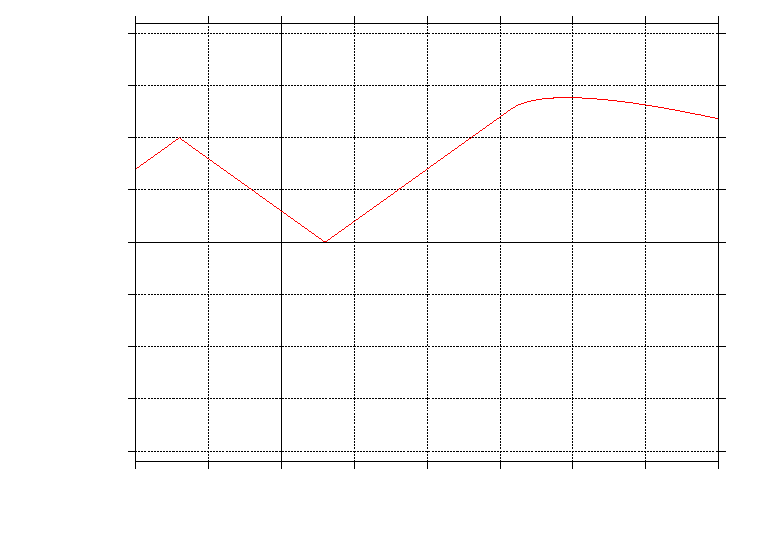
\includegraphics{Edepend}}%
    \gplfronttext
  \end{picture}%
\endgroup
  
\caption{The ground state energy for zero tempetature, $E_0$, is plotted as a function of the interwire distance, $d$. Black dashed: intrawire pairing only, independent of $d$. Black dash-dotted: interwire pairing only, monotonically increasing. In red: $\Delta^{12}_k$ imaginary. In blue: $\Delta^{12}_k$ real. For the free gas: $E_0/\epsilon_{F,0}N_F = 2/3 = 0.667$. Notice that the system with an imaginary interwire pairing is energetically favourable around the critical distance, $d_c$, where the dashed and dash-dotted line intersects. \\
Parameters: $(n_Ba_B^3)^{1/3} = 0.01$, $(n_Ba_{BF}^3)^{1/3} = 0.1$, $l_t = 0$, $m_B / m_F = 7/40$, $n_F / n_B^{1/3} = 0.215$, $v_F/c_0 = 0.33$. }  
\label{fig.2wiresE0ddepend}  
\vspace{0.5cm}
% GNUPLOT: LaTeX picture with Postscript
\begingroup
  \makeatletter
  \providecommand\color[2][]{%
    \GenericError{(gnuplot) \space\space\space\@spaces}{%
      Package color not loaded in conjunction with
      terminal option `colourtext'%
    }{See the gnuplot documentation for explanation.%
    }{Either use 'blacktext' in gnuplot or load the package
      color.sty in LaTeX.}%
    \renewcommand\color[2][]{}%
  }%
  \providecommand\includegraphics[2][]{%
    \GenericError{(gnuplot) \space\space\space\@spaces}{%
      Package graphicx or graphics not loaded%
    }{See the gnuplot documentation for explanation.%
    }{The gnuplot epslatex terminal needs graphicx.sty or graphics.sty.}%
    \renewcommand\includegraphics[2][]{}%
  }%
  \providecommand\rotatebox[2]{#2}%
  \@ifundefined{ifGPcolor}{%
    \newif\ifGPcolor
    \GPcolorfalse
  }{}%
  \@ifundefined{ifGPblacktext}{%
    \newif\ifGPblacktext
    \GPblacktexttrue
  }{}%
  % define a \g@addto@macro without @ in the name:
  \let\gplgaddtomacro\g@addto@macro
  % define empty templates for all commands taking text:
  \gdef\gplbacktext{}%
  \gdef\gplfronttext{}%
  \makeatother
  \ifGPblacktext
    % no textcolor at all
    \def\colorrgb#1{}%
    \def\colorgray#1{}%
  \else
    % gray or color?
    \ifGPcolor
      \def\colorrgb#1{\color[rgb]{#1}}%
      \def\colorgray#1{\color[gray]{#1}}%
      \expandafter\def\csname LTw\endcsname{\color{white}}%
      \expandafter\def\csname LTb\endcsname{\color{black}}%
      \expandafter\def\csname LTa\endcsname{\color{black}}%
      \expandafter\def\csname LT0\endcsname{\color[rgb]{1,0,0}}%
      \expandafter\def\csname LT1\endcsname{\color[rgb]{0,1,0}}%
      \expandafter\def\csname LT2\endcsname{\color[rgb]{0,0,1}}%
      \expandafter\def\csname LT3\endcsname{\color[rgb]{1,0,1}}%
      \expandafter\def\csname LT4\endcsname{\color[rgb]{0,1,1}}%
      \expandafter\def\csname LT5\endcsname{\color[rgb]{1,1,0}}%
      \expandafter\def\csname LT6\endcsname{\color[rgb]{0,0,0}}%
      \expandafter\def\csname LT7\endcsname{\color[rgb]{1,0.3,0}}%
      \expandafter\def\csname LT8\endcsname{\color[rgb]{0.5,0.5,0.5}}%
    \else
      % gray
      \def\colorrgb#1{\color{black}}%
      \def\colorgray#1{\color[gray]{#1}}%
      \expandafter\def\csname LTw\endcsname{\color{white}}%
      \expandafter\def\csname LTb\endcsname{\color{black}}%
      \expandafter\def\csname LTa\endcsname{\color{black}}%
      \expandafter\def\csname LT0\endcsname{\color{black}}%
      \expandafter\def\csname LT1\endcsname{\color{black}}%
      \expandafter\def\csname LT2\endcsname{\color{black}}%
      \expandafter\def\csname LT3\endcsname{\color{black}}%
      \expandafter\def\csname LT4\endcsname{\color{black}}%
      \expandafter\def\csname LT5\endcsname{\color{black}}%
      \expandafter\def\csname LT6\endcsname{\color{black}}%
      \expandafter\def\csname LT7\endcsname{\color{black}}%
      \expandafter\def\csname LT8\endcsname{\color{black}}%
    \fi
  \fi
    \setlength{\unitlength}{0.0500bp}%
    \ifx\gptboxheight\undefined%
      \newlength{\gptboxheight}%
      \newlength{\gptboxwidth}%
      \newsavebox{\gptboxtext}%
    \fi%
    \setlength{\fboxrule}{0.5pt}%
    \setlength{\fboxsep}{1pt}%
\begin{picture}(7200.00,5040.00)%
    \gplgaddtomacro\gplbacktext{%
      \csname LTb\endcsname%
      \put(814,767){\makebox(0,0)[r]{\strut{}$0$}}%
      \csname LTb\endcsname%
      \put(814,1469){\makebox(0,0)[r]{\strut{}$0.1$}}%
      \csname LTb\endcsname%
      \put(814,2170){\makebox(0,0)[r]{\strut{}$0.2$}}%
      \csname LTb\endcsname%
      \put(814,2872){\makebox(0,0)[r]{\strut{}$0.3$}}%
      \csname LTb\endcsname%
      \put(814,3573){\makebox(0,0)[r]{\strut{}$0.4$}}%
      \csname LTb\endcsname%
      \put(814,4275){\makebox(0,0)[r]{\strut{}$0.5$}}%
      \csname LTb\endcsname%
      \put(814,4976){\makebox(0,0)[r]{\strut{}$0.6$}}%
      \csname LTb\endcsname%
      \put(1009,484){\makebox(0,0){\strut{}$0.71$}}%
      \csname LTb\endcsname%
      \put(1828,484){\makebox(0,0){\strut{}$0.72$}}%
      \csname LTb\endcsname%
      \put(2646,484){\makebox(0,0){\strut{}$0.73$}}%
      \csname LTb\endcsname%
      \put(3465,484){\makebox(0,0){\strut{}$0.74$}}%
      \csname LTb\endcsname%
      \put(4284,484){\makebox(0,0){\strut{}$0.75$}}%
      \csname LTb\endcsname%
      \put(5103,484){\makebox(0,0){\strut{}$0.76$}}%
      \csname LTb\endcsname%
      \put(5921,484){\makebox(0,0){\strut{}$0.77$}}%
      \csname LTb\endcsname%
      \put(6740,484){\makebox(0,0){\strut{}$0.78$}}%
    }%
    \gplgaddtomacro\gplfronttext{%
      \csname LTb\endcsname%
      \put(176,2871){\rotatebox{-270}{\makebox(0,0){\strut{}$Delta_k/epsilon_{F,0}$}}}%
      \put(3874,154){\makebox(0,0){\strut{}$k_Fd$}}%
      \csname LTb\endcsname%
      \put(3385,4803){\makebox(0,0)[r]{\strut{}$Intrawire pairing$}}%
      \csname LTb\endcsname%
      \put(3385,4583){\makebox(0,0)[r]{\strut{}$Interwire pairing$}}%
    }%
    \gplbacktext
    \put(0,0){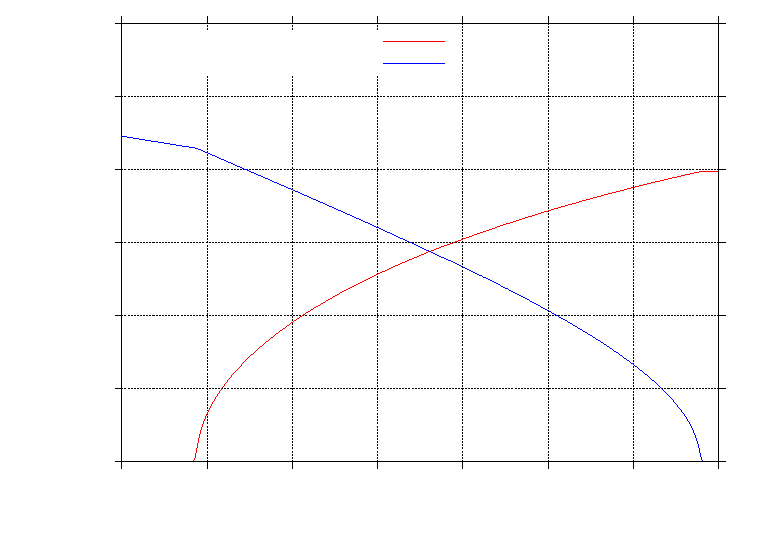
\includegraphics{ddepend}}%
    \gplfronttext
  \end{picture}%
\endgroup
  
\caption{The pairings at the Fermi momentum, $\left|\Delta^{11}_{k_F}\right|$ and $\left|\Delta^{12}_{k_F}\right|$, as a function of the distance $d$ between the wires. In red: pairings for $\Delta^{12}_k$ imaginary, corresponding to the red graph in figure \ref{fig.2wiresE0ddepend}. In blue: Pairings for $\Delta^{12}_k$ real, corresponding to the blue graph in figure \ref{fig.2wiresE0ddepend}. The \textit{inter}wire pairings are shown with dashed lines and are large for small distances. The \textit{intra}wire pairings are shown in solid, and are large for large distances. \\
Parameters: $(n_Ba_B^3)^{1/3} = 0.01$, $(n_Ba_{BF}^3)^{1/3} = 0.1$, $l_t = 0$, $m_B / m_F = 7/40$, $n_F / n_B^{1/3} = 0.215$, $v_F/c_0 = 0.33$. }
\label{fig.2wiresMaximalPairingddepend}
\end{center}
\end{figure}

\subsection{\texorpdfstring{$\Delta^{12}$}{Interwire pairing} real}
In this third case we search for a coexistence of intra- and interwire pairing with the latter, $\Delta^{12}$, being \textit{real}. In this case the system has a time reversal symmetry $T^2 = -\mathbb{I}$, as shown in subsection \ref{subsec.TRwireexchange}. The behaviour of the pairings in this case turn out to be exactly the one described in the previous subsection. This is the blue curve in figure \ref{fig.2wiresE0ddepend}. We are thus \textit{not} able to find a coexistence of intra- and interwire pairing, when the interwire pairing is real. The pairings at the Fermi momentum, $|\Delta^{11}_{k_F}|$ and $|\Delta^{12}_{k_F}|$, are plotted as the blue curves in figure \ref{fig.2wiresMaximalPairingddepend}. Since the pairings are discontinuous at the critical distance, $d_c$, the system experiences a \textit{first} order phase transition between a topological $p$-wave and trivial $s$-wave phase. It is not clear from the gap equations, why we observe this discontinuous behaviour. It is therefore quite a nontrivial result.  

\subsection{\texorpdfstring{$\Delta^{12}$}{Interwire pairing} imaginary}
In this fourth case we again search for a coexistence of intra- and interwire pairing. This time around the latter, $\Delta^{12}$, is imaginary. This corresponds to a breaking of the $T^2 = -\mathbb{I}$ time reversal symmetry. The system still has a $T^2 = + \mathbb{I}$ symmetry. The energy dispersions are identical and even in $k$: $E^{\pm}_{F,k} = E_{F,k} = \sqrt{\varepsilon_k^2 + (\Delta^{11}_k)^2 + |\Delta^{12}_k|^2}$, see figure \ref{fig.Dispersionexamples} for details. This means that the gap equations \eqref{eq.2wiresgapequations} partially decouple: 
\begin{align}
\Delta^{11}_k &= -\frac{1}{\mathcal{L}}\sum_{k'} W_{\text{ind}}^{11}(k, k')\frac{\Delta^{11}_{k'}}{2E_{F,k'}}\tanh\left[\frac{\beta E_{F,k'}}{2}\right], \nonumber \\
\Delta^{12}_k &= -\frac{1}{\mathcal{L}}\sum_{k'} W_{\text{ind}}^{12}(k, k')\frac{\Delta^{12}_{k'}}{2E_{F,k'}}\tanh\left[\frac{\beta E_{F,k'}}{2}\right].
\label{eq.2wiresgapequationsDelta12imaginary}
\end{align} 
This explicitly shows that the two pairings are only coupled through the energy $E_{F,k}$. We start the analysis around the critical distance, $d = d_c$, since both pairings are suspected to be present there. For each value of the interwire distance, $d$, we do something very similar to the above. However, here we do not reinitiate the initial guess in each step of $d$. Instead we reuse the found solution from the previous value of $d$. This makes the analysis much faster, and as long as the pairings are continuous no mistake is made. The result for the energy results in the red curve in figure \ref{fig.2wiresE0ddepend}. We clearly see that this choice of the phase of $\Delta^{12}$ is energetically favourable. Further, we record the pairings at the Fermi momentum as above. The result is shown as the red curves in figure \ref{fig.2wiresMaximalPairingddepend}. Since the pairings are continuous during the transition, but their derivatives are not, the system in this case experiences a \textit{second} order phase transition. From figure \ref{fig.2wiresedgestates} we see that the edge states hereby become gradually gapped. 

The more detailed behaviour of the pairings is to be expected. Naively it seems to be the case that the interwire pairing increases linearly for small interwire distances, $k_Fd < 0.745$. However, an analysis to lower values of $d$ shows that it diverges for $d \to 0$ which is to be expected since the interwire interaction diverges in this limit. We notice that the intrawire pairing is constant from just above $k_Fd = 0.77$ and upwards. This constant behaviour of the intrawire pairing is an artefact of mean field theory. We have not taken the so-called Hartree-Fock energies into account. See section \ref{sec.physicaldiscrepancies} for a further discussion on the matter. We will return to the functional form of the pairings in section \ref{sec.pairingsfunctionalbehaviour} which will explicitly verify that the pairings are in fact $p$- and $s$-wave type.  


\section{Topological invariants}
In this section we investigate in more detail the topological consequences of our numerical results. 

We know from chapter \ref{Chapter5} that an imaginary interwire pairing, $\Delta^{12}$, describes a topologically trivial phase. In this case the $T^2 = -\mathbb{I}$ symmetry is broken and there is only a $T^2 = +\mathbb{I}$ symmetry with a topological invariant, $\nu_{\mathbb{Z}} = 0$. Hence, there are no gapless edge states. To show this explicitly we plot the subsystem ``invariant'' $2\text{CS}_{1,1}$ in figure \ref{fig.2wiresCS11ddepend}. In the case of an imaginary interwire pairing, we observe the following. For large distances, $k_Fd > 0.77$ for the current set of parameters, only $\Delta^{11}$ is present and there is a $T^2 = -\mathbb{I}$ symmetry. Hence, $2\text{CS}_{1,1}$ is a well-defined integer invariant equal to $1$ which is the nontrivial value. Hence, there are gapless edge states. For small distances only $\Delta^{12}$ is present. Here there is also a $T^2 = -\mathbb{I}$ symmetry. Again $2\text{CS}_{1,1}$ is a well-defined invariant, now equal to $0$; the trivial value. There are no gapless edge states. In-between there is a coexistence of intra- and interwire pairing as already discussed. Then $2\text{CS}_{1,1}$ is not well-defined as an integer invariant as noted in section \ref{subsec.2wires_CSinv_Delta12imag}, but it is still a continuous function. In the case of real interwire pairing the topological invariant flips from $1$ to $0$ at the critical distance $d_c$. 

\begin{figure}
\begin{center}
% GNUPLOT: LaTeX picture with Postscript
\begingroup
  \makeatletter
  \providecommand\color[2][]{%
    \GenericError{(gnuplot) \space\space\space\@spaces}{%
      Package color not loaded in conjunction with
      terminal option `colourtext'%
    }{See the gnuplot documentation for explanation.%
    }{Either use 'blacktext' in gnuplot or load the package
      color.sty in LaTeX.}%
    \renewcommand\color[2][]{}%
  }%
  \providecommand\includegraphics[2][]{%
    \GenericError{(gnuplot) \space\space\space\@spaces}{%
      Package graphicx or graphics not loaded%
    }{See the gnuplot documentation for explanation.%
    }{The gnuplot epslatex terminal needs graphicx.sty or graphics.sty.}%
    \renewcommand\includegraphics[2][]{}%
  }%
  \providecommand\rotatebox[2]{#2}%
  \@ifundefined{ifGPcolor}{%
    \newif\ifGPcolor
    \GPcolorfalse
  }{}%
  \@ifundefined{ifGPblacktext}{%
    \newif\ifGPblacktext
    \GPblacktexttrue
  }{}%
  % define a \g@addto@macro without @ in the name:
  \let\gplgaddtomacro\g@addto@macro
  % define empty templates for all commands taking text:
  \gdef\gplbacktext{}%
  \gdef\gplfronttext{}%
  \makeatother
  \ifGPblacktext
    % no textcolor at all
    \def\colorrgb#1{}%
    \def\colorgray#1{}%
  \else
    % gray or color?
    \ifGPcolor
      \def\colorrgb#1{\color[rgb]{#1}}%
      \def\colorgray#1{\color[gray]{#1}}%
      \expandafter\def\csname LTw\endcsname{\color{white}}%
      \expandafter\def\csname LTb\endcsname{\color{black}}%
      \expandafter\def\csname LTa\endcsname{\color{black}}%
      \expandafter\def\csname LT0\endcsname{\color[rgb]{1,0,0}}%
      \expandafter\def\csname LT1\endcsname{\color[rgb]{0,1,0}}%
      \expandafter\def\csname LT2\endcsname{\color[rgb]{0,0,1}}%
      \expandafter\def\csname LT3\endcsname{\color[rgb]{1,0,1}}%
      \expandafter\def\csname LT4\endcsname{\color[rgb]{0,1,1}}%
      \expandafter\def\csname LT5\endcsname{\color[rgb]{1,1,0}}%
      \expandafter\def\csname LT6\endcsname{\color[rgb]{0,0,0}}%
      \expandafter\def\csname LT7\endcsname{\color[rgb]{1,0.3,0}}%
      \expandafter\def\csname LT8\endcsname{\color[rgb]{0.5,0.5,0.5}}%
    \else
      % gray
      \def\colorrgb#1{\color{black}}%
      \def\colorgray#1{\color[gray]{#1}}%
      \expandafter\def\csname LTw\endcsname{\color{white}}%
      \expandafter\def\csname LTb\endcsname{\color{black}}%
      \expandafter\def\csname LTa\endcsname{\color{black}}%
      \expandafter\def\csname LT0\endcsname{\color{black}}%
      \expandafter\def\csname LT1\endcsname{\color{black}}%
      \expandafter\def\csname LT2\endcsname{\color{black}}%
      \expandafter\def\csname LT3\endcsname{\color{black}}%
      \expandafter\def\csname LT4\endcsname{\color{black}}%
      \expandafter\def\csname LT5\endcsname{\color{black}}%
      \expandafter\def\csname LT6\endcsname{\color{black}}%
      \expandafter\def\csname LT7\endcsname{\color{black}}%
      \expandafter\def\csname LT8\endcsname{\color{black}}%
    \fi
  \fi
    \setlength{\unitlength}{0.0500bp}%
    \ifx\gptboxheight\undefined%
      \newlength{\gptboxheight}%
      \newlength{\gptboxwidth}%
      \newsavebox{\gptboxtext}%
    \fi%
    \setlength{\fboxrule}{0.5pt}%
    \setlength{\fboxsep}{1pt}%
\begin{picture}(7200.00,5040.00)%
    \gplgaddtomacro\gplbacktext{%
      \csname LTb\endcsname%
      \put(814,767){\makebox(0,0)[r]{\strut{}$0$}}%
      \csname LTb\endcsname%
      \put(814,1469){\makebox(0,0)[r]{\strut{}$0.2$}}%
      \csname LTb\endcsname%
      \put(814,2170){\makebox(0,0)[r]{\strut{}$0.4$}}%
      \csname LTb\endcsname%
      \put(814,2872){\makebox(0,0)[r]{\strut{}$0.6$}}%
      \csname LTb\endcsname%
      \put(814,3573){\makebox(0,0)[r]{\strut{}$0.8$}}%
      \csname LTb\endcsname%
      \put(814,4275){\makebox(0,0)[r]{\strut{}$1$}}%
      \csname LTb\endcsname%
      \put(814,4976){\makebox(0,0)[r]{\strut{}$1.2$}}%
      \csname LTb\endcsname%
      \put(1009,484){\makebox(0,0){\strut{}$0.74$}}%
      \csname LTb\endcsname%
      \put(1828,484){\makebox(0,0){\strut{}$0.745$}}%
      \csname LTb\endcsname%
      \put(2646,484){\makebox(0,0){\strut{}$0.75$}}%
      \csname LTb\endcsname%
      \put(3465,484){\makebox(0,0){\strut{}$0.755$}}%
      \csname LTb\endcsname%
      \put(4284,484){\makebox(0,0){\strut{}$0.76$}}%
      \csname LTb\endcsname%
      \put(5103,484){\makebox(0,0){\strut{}$0.765$}}%
      \csname LTb\endcsname%
      \put(5921,484){\makebox(0,0){\strut{}$0.77$}}%
      \csname LTb\endcsname%
      \put(6740,484){\makebox(0,0){\strut{}$0.775$}}%
    }%
    \gplgaddtomacro\gplfronttext{%
      \csname LTb\endcsname%
      \put(176,2871){\rotatebox{-270}{\makebox(0,0){\strut{}$2\text{CS}_{1,1}$}}}%
      \put(3874,154){\makebox(0,0){\strut{}$k_Fd$}}%
      \csname LTb\endcsname%
      \put(3047,4803){\makebox(0,0)[l]{\strut{}Interwire pairing imaginary}}%
      \csname LTb\endcsname%
      \put(3047,4583){\makebox(0,0)[l]{\strut{}Interwire pairing real}}%
    }%
    \gplbacktext
    \put(0,0){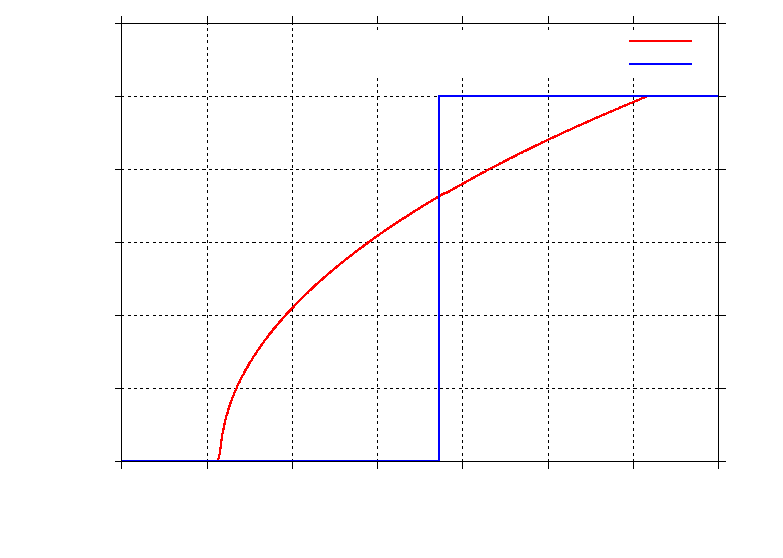
\includegraphics{Figures/twowires/DeltasCS11/CS11depend}}%
    \gplfronttext
  \end{picture}%
\endgroup
  
\caption{The subsystem topological "invariant" $2\text{CS}_{1,1}$. $\text{CS}_{1,2} = - \text{CS}_{1,1}$. In red: $\Delta^{12}_k$ imaginary. For coexistence of $\Delta^{11}_k$ and $\Delta^{12}_k$, $\text{CS}_{1,1}$ is \textit{not} well-defined as an integer invariant. Then it is simply a continuous function which can take any value. In blue: $\Delta^{12}_k$ real. The invariant jumps at the critical distance, $d_c$. \\
Parameters: $(n_Ba_B^3)^{1/3} = 0.01$, $(n_Ba_{BF}^3)^{1/3} = 0.1$, $l_t = 0$, $m_B / m_F = 7/40$, $n_F / n_B^{1/3} = 0.215$, $v_F/c_0 = 0.33$. }  
\label{fig.2wiresCS11ddepend}
\end{center}    
\end{figure} 

As noted above the $\mathbb{Z}$ topological invariant, $\nu_{\mathbb{Z}}$, vanishes identically in the case of imaginary interwire pairing, $\Delta^{12}$. However, in this statement there is an interesting subtlety. To explain this subtlety consider the two wires as uncoupled. In chapter \ref{Chapter4} we chose the gauge $\Delta^{22} = - \Delta^{11}$. In turn we found in chapter \ref{Chapter5} that the winding numbers of each wire $w_j = 2\text{CS}_{1,j}$ differ in sign. However, if we instead choose the gauge where the intrawire pairings are identical, $\Delta^{22} = + \Delta^{11}$, one should then think that the winding numbers for each wire is the same and thus the total winding number would be $\nu_{\mathbb{Z}} = \pm 2$. Hence, it seems that by making a simple gauge transformation we have altered the topological index for the system. A more detailed and careful analysis illuminates this apparent paradox. For the uncoupled wires with $\Delta^{22} = + \Delta^{11}$ it is \textit{possible} to define a set of eigenvectors such that the winding numbers are in fact the same and $\nu_{\mathbb{Z}} = \pm 2$. However, it turns out that this set of eigenvectors is \textit{not} continuously connected to the set defined for nonzero interwire pairings, $\Delta^{12}$. In fact the two sets differ by an overall phase which is discontinuous in $k = 0$. The set of eigenvectors that works for nonzero $\Delta^{12}$ gives the same result as in the originally chosen gauge $\Delta^{22} = - \Delta^{11}$, i.e. the total winding number is $\nu_{\mathbb{Z}} = 0$. The difference in winding number is due to the discontinuous phase connecting the two sets. Hence, we understand this subtlety in the following manner. When the two wires are truly uncoupled it is possible to define two different sets of eigenvectors. One gives a total winding number of $\pm 2$, the other winding number $0$. Since the wires are uncoupled no physical distinction can be made between these values. However, when we allow for a coupling through $\Delta^{12}$ between the two wires, we must choose the set of eigenvectors which is continuous for all $\Delta^{12}$. Then we \textit{can} physically distinguish between the two windings and the correct one is $\nu_{\mathbb{Z}} = 0$. 

The combined result of the figures of the last two sections is the following. For long interwire distances, we have the uncoupled Kitaev wires both with nontrivial topological properties - i.e. there is an edge state present in each wire. For short distances, we have a topologically trivial $s$-wave superfluid and no edge states. For $\Delta^{12}$ imaginary and intermediate interwire distances we find coexistence of the $s$- and $p$-wave pairing. This transition is energetically favourable. It breaks the $T^2 = -\mathbb{I}$ symmetry and leads to gapped edge states. It is a second order phase transition between a topological $p$-wave and trivial $s$-wave phase. This is one of the main results of the thesis. 

Further, for the real interwire pairing we have not been able to find a continuous transition. The pairing simply flips from $p$- to $s$-wave in a discontinuous manner precisely at the critical distance, $d = d_c$, i.e. a first order phase transition. This transition is \textit{not} energetically favourable. 

\section{Pairings: Momentum dependency} \label{sec.pairingsfunctionalbehaviour}
In this section we calculate the momentum dependency of the pairings for the energetically favourable transition. We thus verify that we have indeed found $p$- and $s$-wave solutions. The analysis is performed in the same manner as in section \ref{sec.2wiresCrossover_energy}.

We numerically find self-consistent solutions to the above gap equations \eqref{eq.2wiresgapequationsDelta12imaginary} along with the number equation \eqref{eq.2wiresnumberequation} as described in the previous section. This is summarized in figure \ref{fig.pairingkdependT0dvaried} for several values of the interwire distance, $d$. We observe an odd \textit{intra}wire $p$-wave pairing as required by Fermi anti-symmetry and an even \textit{inter}wire $s$-wave pairing. The pairings show no oscillatory behaviour, they simply decay for large values of $k$. The $p$-wave pairing decays in a power-law fashion and is well-described by a function on the form $k / (k^2 + a)$. The $s$-wave pairing decays exponentially fast. The overall behaviour of the pairings are seen to be independent of the interwire distance, $d$. The interwire pairing is simply enhanced as $d$ decreases, vice versa for the intrawire pairing.  

\begin{figure} 
\begin{center}  
% GNUPLOT: LaTeX picture with Postscript
\begingroup
  \makeatletter
  \providecommand\color[2][]{%
    \GenericError{(gnuplot) \space\space\space\@spaces}{%
      Package color not loaded in conjunction with
      terminal option `colourtext'%
    }{See the gnuplot documentation for explanation.%
    }{Either use 'blacktext' in gnuplot or load the package
      color.sty in LaTeX.}%
    \renewcommand\color[2][]{}%
  }%
  \providecommand\includegraphics[2][]{%
    \GenericError{(gnuplot) \space\space\space\@spaces}{%
      Package graphicx or graphics not loaded%
    }{See the gnuplot documentation for explanation.%
    }{The gnuplot epslatex terminal needs graphicx.sty or graphics.sty.}%
    \renewcommand\includegraphics[2][]{}%
  }%
  \providecommand\rotatebox[2]{#2}%
  \@ifundefined{ifGPcolor}{%
    \newif\ifGPcolor
    \GPcolorfalse
  }{}%
  \@ifundefined{ifGPblacktext}{%
    \newif\ifGPblacktext
    \GPblacktexttrue
  }{}%
  % define a \g@addto@macro without @ in the name:
  \let\gplgaddtomacro\g@addto@macro
  % define empty templates for all commands taking text:
  \gdef\gplbacktext{}%
  \gdef\gplfronttext{}%
  \makeatother
  \ifGPblacktext
    % no textcolor at all
    \def\colorrgb#1{}%
    \def\colorgray#1{}%
  \else
    % gray or color?
    \ifGPcolor
      \def\colorrgb#1{\color[rgb]{#1}}%
      \def\colorgray#1{\color[gray]{#1}}%
      \expandafter\def\csname LTw\endcsname{\color{white}}%
      \expandafter\def\csname LTb\endcsname{\color{black}}%
      \expandafter\def\csname LTa\endcsname{\color{black}}%
      \expandafter\def\csname LT0\endcsname{\color[rgb]{1,0,0}}%
      \expandafter\def\csname LT1\endcsname{\color[rgb]{0,1,0}}%
      \expandafter\def\csname LT2\endcsname{\color[rgb]{0,0,1}}%
      \expandafter\def\csname LT3\endcsname{\color[rgb]{1,0,1}}%
      \expandafter\def\csname LT4\endcsname{\color[rgb]{0,1,1}}%
      \expandafter\def\csname LT5\endcsname{\color[rgb]{1,1,0}}%
      \expandafter\def\csname LT6\endcsname{\color[rgb]{0,0,0}}%
      \expandafter\def\csname LT7\endcsname{\color[rgb]{1,0.3,0}}%
      \expandafter\def\csname LT8\endcsname{\color[rgb]{0.5,0.5,0.5}}%
    \else
      % gray
      \def\colorrgb#1{\color{black}}%
      \def\colorgray#1{\color[gray]{#1}}%
      \expandafter\def\csname LTw\endcsname{\color{white}}%
      \expandafter\def\csname LTb\endcsname{\color{black}}%
      \expandafter\def\csname LTa\endcsname{\color{black}}%
      \expandafter\def\csname LT0\endcsname{\color{black}}%
      \expandafter\def\csname LT1\endcsname{\color{black}}%
      \expandafter\def\csname LT2\endcsname{\color{black}}%
      \expandafter\def\csname LT3\endcsname{\color{black}}%
      \expandafter\def\csname LT4\endcsname{\color{black}}%
      \expandafter\def\csname LT5\endcsname{\color{black}}%
      \expandafter\def\csname LT6\endcsname{\color{black}}%
      \expandafter\def\csname LT7\endcsname{\color{black}}%
      \expandafter\def\csname LT8\endcsname{\color{black}}%
    \fi
  \fi
    \setlength{\unitlength}{0.0500bp}%
    \ifx\gptboxheight\undefined%
      \newlength{\gptboxheight}%
      \newlength{\gptboxwidth}%
      \newsavebox{\gptboxtext}%
    \fi%
    \setlength{\fboxrule}{0.5pt}%
    \setlength{\fboxsep}{1pt}%
\begin{picture}(7200.00,5040.00)%
    \gplgaddtomacro\gplbacktext{%
      \csname LTb\endcsname%
      \put(946,767){\makebox(0,0)[r]{\strut{}$-0.3$}}%
      \csname LTb\endcsname%
      \put(946,1468){\makebox(0,0)[r]{\strut{}$-0.2$}}%
      \csname LTb\endcsname%
      \put(946,2170){\makebox(0,0)[r]{\strut{}$-0.1$}}%
      \csname LTb\endcsname%
      \put(946,2871){\makebox(0,0)[r]{\strut{}$0$}}%
      \csname LTb\endcsname%
      \put(946,3573){\makebox(0,0)[r]{\strut{}$0.1$}}%
      \csname LTb\endcsname%
      \put(946,4275){\makebox(0,0)[r]{\strut{}$0.2$}}%
      \csname LTb\endcsname%
      \put(946,4976){\makebox(0,0)[r]{\strut{}$0.3$}}%
      \csname LTb\endcsname%
      \put(1141,484){\makebox(0,0){\strut{}$-10$}}%
      \csname LTb\endcsname%
      \put(2541,484){\makebox(0,0){\strut{}$-5$}}%
      \csname LTb\endcsname%
      \put(3941,484){\makebox(0,0){\strut{}$0$}}%
      \csname LTb\endcsname%
      \put(5340,484){\makebox(0,0){\strut{}$5$}}%
      \csname LTb\endcsname%
      \put(6740,484){\makebox(0,0){\strut{}$10$}}%
    }%
    \gplgaddtomacro\gplfronttext{%
      \csname LTb\endcsname%
      \put(176,2871){\rotatebox{-270}{\makebox(0,0){\strut{}$\Delta_k/\epsilon_{F,0}$}}}%
      \put(3940,154){\makebox(0,0){\strut{}$k/k_F$}}%
      \csname LTb\endcsname%
      \put(4275,1820){\makebox(0,0)[l]{\strut{}$k_Fd = 0.7475$}}%
      \csname LTb\endcsname%
      \put(4275,1600){\makebox(0,0)[l]{\strut{}$k_Fd = 0.7525$}}%
      \csname LTb\endcsname%
      \put(4275,1380){\makebox(0,0)[l]{\strut{}$k_Fd = 0.7575$}}%
      \csname LTb\endcsname%
      \put(4275,1160){\makebox(0,0)[l]{\strut{}$k_Fd = 0.7625$}}%
      \csname LTb\endcsname%
      \put(4275,940){\makebox(0,0)[l]{\strut{}$k_Fd = 0.7675$}}%
    }%
    \gplbacktext
    \put(0,0){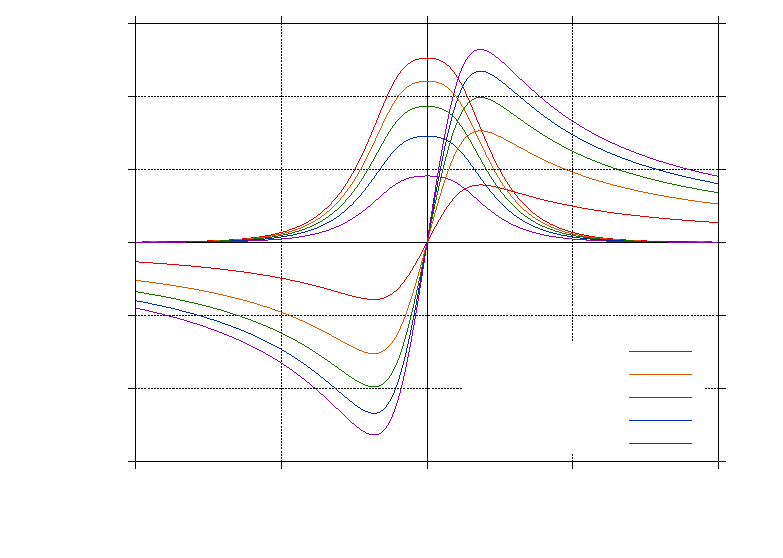
\includegraphics{Figures/twowires/Deltas1.0/kdepend}}%
    \gplfronttext
  \end{picture}%
\endgroup
  
\caption{The pairings $\Delta^{11}_k$ (odd) and $\Delta^{12}_k$ (even) plotted as a function of $k$ for $\Delta^{12}_k$ imaginary. We see that the functional behaviour is independent of $d$ and that there is a transition between interwire and intrawire dominated pairing. The intrawire pairing is increased as $d$ increases. Vice versa for the interwire pairing. \\
Parameters: $(n_Ba_B^3)^{1/3} = 0.01$, $(n_Ba_{BF}^3)^{1/3} = 0.1$, $l_t = 0$, $m_B / m_F = 7/40$, $n_F / n_B^{1/3} = 0.215$, $v_F / c_0 = 0.33$. }  
\label{fig.pairingkdependT0dvaried}  
\end{center}    
\end{figure}

In appendix \ref{Appendix.pairingtemperaturedependency} we have calculated the pairings as a function of temperature at the critical distance $k_Fd_c = 0.759$ for the current set of parameters. The temperature dependency is consistent with Landau's theory of phase transitions as described in section \ref{sec.landauphasetransitions}, where the pairings go to zero at two different critical temperatures, $T_c$. For the uncoupled wires we study the criticial temperature of the intrawire pairing within our current formalism in appendix \ref{Appendix.criticaltemperature}. However, the behaviour for nonzero temperatures is highly unreliable due to the increasing phase fluctuations with increasing temperature. Significant steps beyond our current formalism must be taken to come with more reliable calculations of the temperature dependency. This is the reason for omitting the seresults in the main text. We will not pursue the behaviour for nonzero temperatures any further.


\section{Pair wave functions} \label{sec.pairwavefunctions}
To get a physically clearer picture of the nature of the pairings we calculate the pair wave functions in real space. These are correlation functions, $\braket{\psi_{i,F}(x')\psi_{j,F}(x)}$ that describe how two fermions are correlated as a function of there respective positions. Specifically, a high absolute value of $\braket{\psi_{i,F}(x')\psi_{j,F}(x)}$ means that the fermions have a tendency to be at those positions $x$ and $x'$. This is the reason why we refer to them as pair wave functions. However, caution should be taken, since the correlation functions are not a direct measure of probability. 

\begin{figure} 
\begin{center}  
% GNUPLOT: LaTeX picture with Postscript
\begingroup
  \makeatletter
  \providecommand\color[2][]{%
    \GenericError{(gnuplot) \space\space\space\@spaces}{%
      Package color not loaded in conjunction with
      terminal option `colourtext'%
    }{See the gnuplot documentation for explanation.%
    }{Either use 'blacktext' in gnuplot or load the package
      color.sty in LaTeX.}%
    \renewcommand\color[2][]{}%
  }%
  \providecommand\includegraphics[2][]{%
    \GenericError{(gnuplot) \space\space\space\@spaces}{%
      Package graphicx or graphics not loaded%
    }{See the gnuplot documentation for explanation.%
    }{The gnuplot epslatex terminal needs graphicx.sty or graphics.sty.}%
    \renewcommand\includegraphics[2][]{}%
  }%
  \providecommand\rotatebox[2]{#2}%
  \@ifundefined{ifGPcolor}{%
    \newif\ifGPcolor
    \GPcolorfalse
  }{}%
  \@ifundefined{ifGPblacktext}{%
    \newif\ifGPblacktext
    \GPblacktexttrue
  }{}%
  % define a \g@addto@macro without @ in the name:
  \let\gplgaddtomacro\g@addto@macro
  % define empty templates for all commands taking text:
  \gdef\gplbacktext{}%
  \gdef\gplfronttext{}%
  \makeatother
  \ifGPblacktext
    % no textcolor at all
    \def\colorrgb#1{}%
    \def\colorgray#1{}%
  \else
    % gray or color?
    \ifGPcolor
      \def\colorrgb#1{\color[rgb]{#1}}%
      \def\colorgray#1{\color[gray]{#1}}%
      \expandafter\def\csname LTw\endcsname{\color{white}}%
      \expandafter\def\csname LTb\endcsname{\color{black}}%
      \expandafter\def\csname LTa\endcsname{\color{black}}%
      \expandafter\def\csname LT0\endcsname{\color[rgb]{1,0,0}}%
      \expandafter\def\csname LT1\endcsname{\color[rgb]{0,1,0}}%
      \expandafter\def\csname LT2\endcsname{\color[rgb]{0,0,1}}%
      \expandafter\def\csname LT3\endcsname{\color[rgb]{1,0,1}}%
      \expandafter\def\csname LT4\endcsname{\color[rgb]{0,1,1}}%
      \expandafter\def\csname LT5\endcsname{\color[rgb]{1,1,0}}%
      \expandafter\def\csname LT6\endcsname{\color[rgb]{0,0,0}}%
      \expandafter\def\csname LT7\endcsname{\color[rgb]{1,0.3,0}}%
      \expandafter\def\csname LT8\endcsname{\color[rgb]{0.5,0.5,0.5}}%
    \else
      % gray
      \def\colorrgb#1{\color{black}}%
      \def\colorgray#1{\color[gray]{#1}}%
      \expandafter\def\csname LTw\endcsname{\color{white}}%
      \expandafter\def\csname LTb\endcsname{\color{black}}%
      \expandafter\def\csname LTa\endcsname{\color{black}}%
      \expandafter\def\csname LT0\endcsname{\color{black}}%
      \expandafter\def\csname LT1\endcsname{\color{black}}%
      \expandafter\def\csname LT2\endcsname{\color{black}}%
      \expandafter\def\csname LT3\endcsname{\color{black}}%
      \expandafter\def\csname LT4\endcsname{\color{black}}%
      \expandafter\def\csname LT5\endcsname{\color{black}}%
      \expandafter\def\csname LT6\endcsname{\color{black}}%
      \expandafter\def\csname LT7\endcsname{\color{black}}%
      \expandafter\def\csname LT8\endcsname{\color{black}}%
    \fi
  \fi
    \setlength{\unitlength}{0.0500bp}%
    \ifx\gptboxheight\undefined%
      \newlength{\gptboxheight}%
      \newlength{\gptboxwidth}%
      \newsavebox{\gptboxtext}%
    \fi%
    \setlength{\fboxrule}{0.5pt}%
    \setlength{\fboxsep}{1pt}%
\begin{picture}(7200.00,5040.00)%
    \gplgaddtomacro\gplbacktext{%
      \csname LTb\endcsname%
      \put(1078,1118){\makebox(0,0)[r]{\strut{}$-0.1$}}%
      \csname LTb\endcsname%
      \put(1078,1995){\makebox(0,0)[r]{\strut{}$-0.05$}}%
      \csname LTb\endcsname%
      \put(1078,2871){\makebox(0,0)[r]{\strut{}$0$}}%
      \csname LTb\endcsname%
      \put(1078,3748){\makebox(0,0)[r]{\strut{}$0.05$}}%
      \csname LTb\endcsname%
      \put(1078,4625){\makebox(0,0)[r]{\strut{}$0.1$}}%
      \csname LTb\endcsname%
      \put(1273,484){\makebox(0,0){\strut{}$-15$}}%
      \csname LTb\endcsname%
      \put(2184,484){\makebox(0,0){\strut{}$-10$}}%
      \csname LTb\endcsname%
      \put(3095,484){\makebox(0,0){\strut{}$-5$}}%
      \csname LTb\endcsname%
      \put(4007,484){\makebox(0,0){\strut{}$0$}}%
      \csname LTb\endcsname%
      \put(4918,484){\makebox(0,0){\strut{}$5$}}%
      \csname LTb\endcsname%
      \put(5829,484){\makebox(0,0){\strut{}$10$}}%
      \csname LTb\endcsname%
      \put(6740,484){\makebox(0,0){\strut{}$15$}}%
    }%
    \gplgaddtomacro\gplfronttext{%
      \csname LTb\endcsname%
      \put(176,2871){\rotatebox{-270}{\makebox(0,0){\strut{}$\braket{ \psi_{1,F}(x)\psi_{1,F}(0) } / k_F$}}}%
      \put(4006,154){\makebox(0,0){\strut{}$k_Fx$}}%
      \csname LTb\endcsname%
      \put(5753,1820){\makebox(0,0)[r]{\strut{}$k_Fd = 0.7475$}}%
      \csname LTb\endcsname%
      \put(5753,1600){\makebox(0,0)[r]{\strut{}$k_Fd = 0.7525$}}%
      \csname LTb\endcsname%
      \put(5753,1380){\makebox(0,0)[r]{\strut{}$k_Fd = 0.7575$}}%
      \csname LTb\endcsname%
      \put(5753,1160){\makebox(0,0)[r]{\strut{}$k_Fd = 0.7625$}}%
      \csname LTb\endcsname%
      \put(5753,940){\makebox(0,0)[r]{\strut{}$k_Fd = 0.7675$}}%
    }%
    \gplbacktext
    \put(0,0){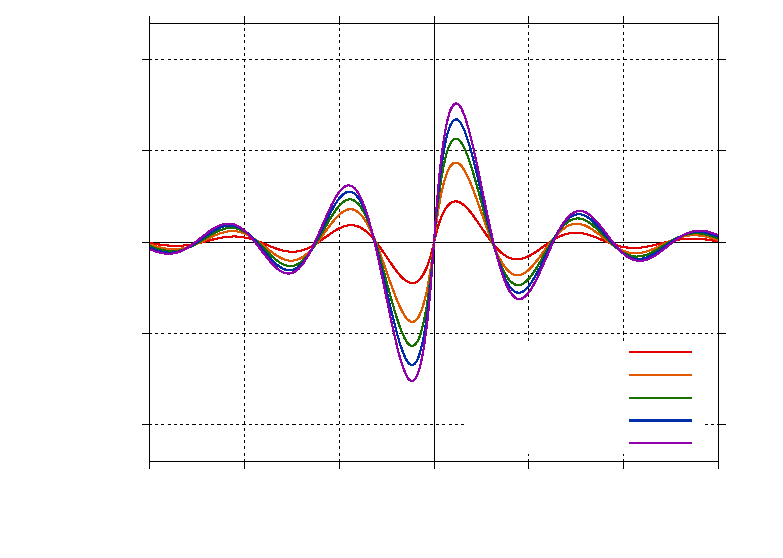
\includegraphics{Figures/twowires/pairwavefunctions1/xdepend11}}%
    \gplfronttext
  \end{picture}%
\endgroup
  
\caption{The \textit{intra}wire pairwave function $\braket{\psi_{1,F}(x)\psi_{1,F}(0)}$ as a function of $x$ for $\Delta^{12}_k$ imaginary. We see that the functional behaviour is independent of $d$, the pair wave function is simply increased as $d$ increases. \\
Parameters: $(n_Ba_B^3)^{1/3} = 0.01$, $(n_Ba_{BF}^3)^{1/3} = 0.1$, $l_t = 0$, $m_B / m_F = 7/40$, $n_F / n_B^{1/3} = 0.215$, $v_F / c_0 = 0.33$. }  
\label{fig.2wirespairwavefunction11}  
\vspace{0.5cm}
% GNUPLOT: LaTeX picture with Postscript
\begingroup
  \makeatletter
  \providecommand\color[2][]{%
    \GenericError{(gnuplot) \space\space\space\@spaces}{%
      Package color not loaded in conjunction with
      terminal option `colourtext'%
    }{See the gnuplot documentation for explanation.%
    }{Either use 'blacktext' in gnuplot or load the package
      color.sty in LaTeX.}%
    \renewcommand\color[2][]{}%
  }%
  \providecommand\includegraphics[2][]{%
    \GenericError{(gnuplot) \space\space\space\@spaces}{%
      Package graphicx or graphics not loaded%
    }{See the gnuplot documentation for explanation.%
    }{The gnuplot epslatex terminal needs graphicx.sty or graphics.sty.}%
    \renewcommand\includegraphics[2][]{}%
  }%
  \providecommand\rotatebox[2]{#2}%
  \@ifundefined{ifGPcolor}{%
    \newif\ifGPcolor
    \GPcolorfalse
  }{}%
  \@ifundefined{ifGPblacktext}{%
    \newif\ifGPblacktext
    \GPblacktexttrue
  }{}%
  % define a \g@addto@macro without @ in the name:
  \let\gplgaddtomacro\g@addto@macro
  % define empty templates for all commands taking text:
  \gdef\gplbacktext{}%
  \gdef\gplfronttext{}%
  \makeatother
  \ifGPblacktext
    % no textcolor at all
    \def\colorrgb#1{}%
    \def\colorgray#1{}%
  \else
    % gray or color?
    \ifGPcolor
      \def\colorrgb#1{\color[rgb]{#1}}%
      \def\colorgray#1{\color[gray]{#1}}%
      \expandafter\def\csname LTw\endcsname{\color{white}}%
      \expandafter\def\csname LTb\endcsname{\color{black}}%
      \expandafter\def\csname LTa\endcsname{\color{black}}%
      \expandafter\def\csname LT0\endcsname{\color[rgb]{1,0,0}}%
      \expandafter\def\csname LT1\endcsname{\color[rgb]{0,1,0}}%
      \expandafter\def\csname LT2\endcsname{\color[rgb]{0,0,1}}%
      \expandafter\def\csname LT3\endcsname{\color[rgb]{1,0,1}}%
      \expandafter\def\csname LT4\endcsname{\color[rgb]{0,1,1}}%
      \expandafter\def\csname LT5\endcsname{\color[rgb]{1,1,0}}%
      \expandafter\def\csname LT6\endcsname{\color[rgb]{0,0,0}}%
      \expandafter\def\csname LT7\endcsname{\color[rgb]{1,0.3,0}}%
      \expandafter\def\csname LT8\endcsname{\color[rgb]{0.5,0.5,0.5}}%
    \else
      % gray
      \def\colorrgb#1{\color{black}}%
      \def\colorgray#1{\color[gray]{#1}}%
      \expandafter\def\csname LTw\endcsname{\color{white}}%
      \expandafter\def\csname LTb\endcsname{\color{black}}%
      \expandafter\def\csname LTa\endcsname{\color{black}}%
      \expandafter\def\csname LT0\endcsname{\color{black}}%
      \expandafter\def\csname LT1\endcsname{\color{black}}%
      \expandafter\def\csname LT2\endcsname{\color{black}}%
      \expandafter\def\csname LT3\endcsname{\color{black}}%
      \expandafter\def\csname LT4\endcsname{\color{black}}%
      \expandafter\def\csname LT5\endcsname{\color{black}}%
      \expandafter\def\csname LT6\endcsname{\color{black}}%
      \expandafter\def\csname LT7\endcsname{\color{black}}%
      \expandafter\def\csname LT8\endcsname{\color{black}}%
    \fi
  \fi
    \setlength{\unitlength}{0.0500bp}%
    \ifx\gptboxheight\undefined%
      \newlength{\gptboxheight}%
      \newlength{\gptboxwidth}%
      \newsavebox{\gptboxtext}%
    \fi%
    \setlength{\fboxrule}{0.5pt}%
    \setlength{\fboxsep}{1pt}%
\begin{picture}(7200.00,5040.00)%
    \gplgaddtomacro\gplbacktext{%
      \csname LTb\endcsname%
      \put(1078,1118){\makebox(0,0)[r]{\strut{}$-0.1$}}%
      \csname LTb\endcsname%
      \put(1078,1995){\makebox(0,0)[r]{\strut{}$-0.05$}}%
      \csname LTb\endcsname%
      \put(1078,2871){\makebox(0,0)[r]{\strut{}$0$}}%
      \csname LTb\endcsname%
      \put(1078,3748){\makebox(0,0)[r]{\strut{}$0.05$}}%
      \csname LTb\endcsname%
      \put(1078,4625){\makebox(0,0)[r]{\strut{}$0.1$}}%
      \csname LTb\endcsname%
      \put(1273,484){\makebox(0,0){\strut{}$-15$}}%
      \csname LTb\endcsname%
      \put(2184,484){\makebox(0,0){\strut{}$-10$}}%
      \csname LTb\endcsname%
      \put(3095,484){\makebox(0,0){\strut{}$-5$}}%
      \csname LTb\endcsname%
      \put(4007,484){\makebox(0,0){\strut{}$0$}}%
      \csname LTb\endcsname%
      \put(4918,484){\makebox(0,0){\strut{}$5$}}%
      \csname LTb\endcsname%
      \put(5829,484){\makebox(0,0){\strut{}$10$}}%
      \csname LTb\endcsname%
      \put(6740,484){\makebox(0,0){\strut{}$15$}}%
    }%
    \gplgaddtomacro\gplfronttext{%
      \csname LTb\endcsname%
      \put(176,2871){\rotatebox{-270}{\makebox(0,0){\strut{}$\braket{\psi_{1,F}(x)\psi_{2,F}(0)}/k_F$}}}%
      \put(4006,154){\makebox(0,0){\strut{}$k_Fx$}}%
      \csname LTb\endcsname%
      \put(5753,1820){\makebox(0,0)[r]{\strut{}$k_Fd = 0.7475$}}%
      \csname LTb\endcsname%
      \put(5753,1600){\makebox(0,0)[r]{\strut{}$k_Fd = 0.7525$}}%
      \csname LTb\endcsname%
      \put(5753,1380){\makebox(0,0)[r]{\strut{}$k_Fd = 0.7575$}}%
      \csname LTb\endcsname%
      \put(5753,1160){\makebox(0,0)[r]{\strut{}$k_Fd = 0.7625$}}%
      \csname LTb\endcsname%
      \put(5753,940){\makebox(0,0)[r]{\strut{}$k_Fd = 0.7675$}}%
    }%
    \gplbacktext
    \put(0,0){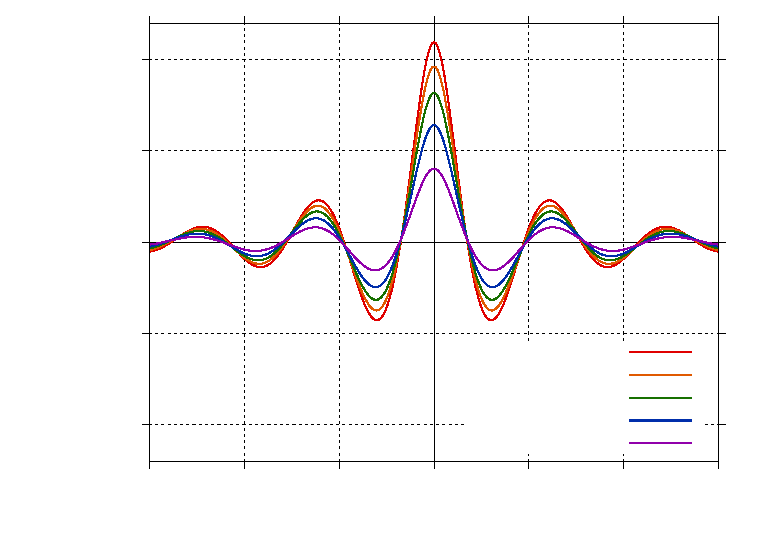
\includegraphics{Figures/twowires/pairwavefunctions1/xdepend12}}%
    \gplfronttext
  \end{picture}%
\endgroup
  
\caption{The \textit{inter}wire pairwave function $\braket{\psi_{1,F}(x)\psi_{2,F}(0)}$ as a function of $x$ for $\Delta^{12}_k$ imaginary. We see that the functional behaviour is independent of $d$, the pair wave function is simply decreased as $d$ increases. \\
Parameters: $(n_Ba_B^3)^{1/3} = 0.01$, $(n_Ba_{BF}^3)^{1/3} = 0.1$, $l_t = 0$, $m_B / m_F = 7/40$, $n_F / n_B^{1/3} = 0.215$, $v_F / c_0 = 0.33$. }  
\label{fig.2wirespairwavefunction12}  
\end{center}    
\end{figure}

We use the Fourier decomposition $\psi_{1,F}(x) = \frac{1}{\sqrt{\mathcal{L}}} \sum_k \text{e}^{ikx} c_{1,k}$ to get an expression for the pair wave functions. For the fermions in wire 1, we get:
\begin{align}
\braket{\psi_{1,F}(x')\psi_{1,F}(x)} 
&= \frac{1}{\mathcal{L}} \sum_{k,q} \text{e}^{i(kx' + qx)}\braket{c_{1,k}c_{1,q}} = \frac{1}{\mathcal{L}} \sum_{k} \text{e}^{ik(x' - x)}\braket{c_{1,k}c_{1,-k}} \nonumber \\
&= \frac{i}{\mathcal{L}} \sum_{k} \sin\left(k(x' - x)\right)\braket{c_{1,k}c_{1,-k}}. \nonumber 
\end{align}
Here we first use that we consider only states, where opposite momenta couples: $q = -k$. Then we use that the fermionic operators anticommute. Hence, $c_{1,k}c_{1,-k}$ is odd in $k$. We notice that it only depends on the difference $x' - x$. We therefore let $x \to 0$ and $x' \to x$. We then insert the mean field of equation \eqref{eq.meanfield11} for $\Delta^{12}_k$ imaginary, and get:
\begin{equation}
\braket{\psi_{1,F}(x)\psi_{1,F}(0)} = - \braket{\psi_{2,F}(x)\psi_{2,F}(0)} = \frac{i}{\mathcal{L}}\sum_k \sin(kx) \frac{\Delta^{11}_k}{2E_{F,k}}\tanh\left[\frac{ \beta E_{F,k} }{2}\right], 
\label{eq.intrawirepairwavefunction}
\end{equation}
The same calculation is carried through for the interwire pair wave function. This gives:
\begin{equation}
\braket{\psi_{1,F}(x)\psi_{2,F}(0)} = \frac{1}{\mathcal{L}}\sum_k \cos(kx) \frac{\Delta^{12}_k}{2E_{F,k}}\tanh\left[\frac{ \beta E_{F,k} }{2}\right].
\label{eq.interwirepairwavefunction}
\end{equation} 
Here we should note that if $E^\pm_{F,k} \neq E_{F,k}$ the above pair wave functions will be altered. From this we can infer an overall functional behaviour. Firstly, we see that $\braket{\psi_{1,F}(x)\psi_{1,F}(0)}$ and $\braket{\psi_{1,F}(x)\psi_{2,F}(0)}$ are respectively odd and even in $x$ which is expexted for $p$- and $s$-wave pairing. Further, $\sin(kx)$ and $\cos(kx)$ oscillate more rapidly as a function of $k$ at higher values of $x$. Therefore, we expect the pair wave functions to decay to 0. This is also physically reasonable: fermions macroscopically far apart should not be correlated. 

\begin{figure}
\center
\begin{tikzpicture}[scale=2/3]
\pgfmathsetmacro{\hmove}{0}
\pgfmathsetmacro{\distance}{2.5}

\node at (3 + \hmove, 4) {Only intrawire};

\coordinate (a1) at (0.5 + \hmove, 0.14);
\coordinate (a2) at (1.6 + \hmove, 0.14);
\coordinate (a3) at (2.4 + \hmove, 0.14);
\coordinate (correlation) at (3.14, 0);

%Bottom:

\draw[-, thick]  (0 + \hmove, 0) -- (6 + \hmove, 0);
\draw[-|, thick] (0 + \hmove, 0) -- (1 + \hmove, 0);
\draw[-|, thick] (1 + \hmove, 0) -- (2 + \hmove, 0);
\draw[-|, thick] (2 + \hmove, 0) -- (3 + \hmove, 0);
\draw[-|, thick] (3 + \hmove, 0) -- (4 + \hmove, 0);
\draw[-|, thick] (4 + \hmove, 0) -- (5 + \hmove, 0);

\draw[*-, semithick] (a1); 
\draw[*-, semithick] (a1) + (correlation);
%correlation 1:
\coordinate (cor11) at (0.5 - 0.2 + \hmove, 0);
\coordinate (cor12) at (3.14 + 0.5 + 0.2 + \hmove , 0);
\draw[-, thick, red]  (cor11) to[out=90, in=90, distance=0.8cm] (cor12);
\draw[-, thick, red]  (cor11) to[out=-90, in=-90, distance=0.8cm] (cor12);

\draw[*-, semithick] (a2);
\draw[*-, semithick] (a2) + (correlation);
%correlation 2 and 4:
\coordinate (cor21) at (1.6 + 0.2 + \hmove, 0);
\coordinate (prior1) at (0 + \hmove,  0.58);
\coordinate (prior2) at (0 + \hmove, -0.58);

\coordinate (cor22) at (1.6 + 3.14 - 0.2 + \hmove , 0);
\coordinate (post1) at (6 + \hmove,  0.58);
\coordinate (post2) at (6 + \hmove, -0.58);

\draw[-, thick, red]  (cor21) to[out= 90, in=0, distance=0.5cm] (prior1);
\draw[-, thick, red]  (cor21) to[out=-90, in=0, distance=0.5cm] (prior2);

\draw[-, thick, red]  (cor22) to[out= 90, in=180, distance=0.45cm] (post1);
\draw[-, thick, red]  (cor22) to[out=-90, in=180, distance=0.45cm] (post2);

\draw[*-, semithick] (a3);
\draw[*-, semithick] (a3) + (correlation);
%correlation 3:
\coordinate (cor31) at (2.4 - 0.2 + \hmove, 0);
\coordinate (cor32) at (2.4 + 3.14 + 0.2 + \hmove, 0);
\draw[-, thick, red]  (cor31) to[out=90, in=90, distance=0.8cm] (cor32);
\draw[-, thick, red]  (cor31) to[out=-90, in=-90, distance=0.8cm] (cor32);


%Top:
\pgfmathsetmacro{\hmovetoppoints}{-0.2}
\coordinate (a1) at (0.5 + \hmove + \hmovetoppoints, 0.14 + \distance);
\coordinate (a2) at (1.6 + \hmove + \hmovetoppoints, 0.14 + \distance);
\coordinate (a3) at (2.4 + \hmove + \hmovetoppoints, 0.14 + \distance);

\draw[-, thick]  (0 + \hmove, 0 + \distance) -- (6 + \hmove, 0 + \distance);
\draw[-|, thick] (0 + \hmove, 0 + \distance) -- (1 + \hmove, 0 + \distance);
\draw[-|, thick] (1 + \hmove, 0 + \distance) -- (2 + \hmove, 0 + \distance);
\draw[-|, thick] (2 + \hmove, 0 + \distance) -- (3 + \hmove, 0 + \distance);
\draw[-|, thick] (3 + \hmove, 0 + \distance) -- (4 + \hmove, 0 + \distance);
\draw[-|, thick] (4 + \hmove, 0 + \distance) -- (5 + \hmove, 0 + \distance);

\draw[*-, semithick] (a1); 
\draw[*-, semithick] (a1) + (correlation);
%correlation 1:
\coordinate (cor11) at (0.5 - 0.2 + \hmove + \hmovetoppoints, 0 + \distance);
\coordinate (cor12) at (3.14 + 0.5 + 0.2 + \hmove + \hmovetoppoints, 0 + \distance);
\draw[-, thick, red]  (cor11) to[out=90, in=90, distance=0.8cm] (cor12);
\draw[-, thick, red]  (cor11) to[out=-90, in=-90, distance=0.8cm] (cor12);

\draw[*-, semithick] (a2);
\draw[*-, semithick] (a2) + (correlation);
%correlation 2 and 4:
\coordinate (cor21) at (1.6 + 0.2 + \hmove + \hmovetoppoints, 0 + \distance);
\coordinate (prior1) at (0 + \hmove,  0.58 + \distance);
\coordinate (prior2) at (0 + \hmove, -0.58 + \distance);

\coordinate (cor22) at (1.6 + 3.14 - 0.2 + \hmove + \hmovetoppoints , 0 + \distance);
\coordinate (post1) at (6 + \hmove,  0.58 + \distance);
\coordinate (post2) at (6 + \hmove, -0.58 + \distance);

\draw[-, thick, red]  (cor21) to[out= 90, in=0, distance=0.45cm] (prior1);
\draw[-, thick, red]  (cor21) to[out=-90, in=0, distance=0.45cm] (prior2);

\draw[-, thick, red]  (cor22) to[out= 90, in=180, distance=0.5cm] (post1);
\draw[-, thick, red]  (cor22) to[out=-90, in=180, distance=0.5cm] (post2);

\draw[*-, semithick] (a3);
\draw[*-, semithick] (a3) + (correlation);
%correlation 3:
\coordinate (cor31) at (2.4 - 0.2 + \hmove + \hmovetoppoints, 0 + \distance);
\coordinate (cor32) at (2.4 + 3.14 + 0.2 + \hmove + \hmovetoppoints, 0 + \distance);
\draw[-, thick, red]  (cor31) to[out=90, in=90, distance=0.8cm] (cor32);
\draw[-, thick, red]  (cor31) to[out=-90, in=-90, distance=0.8cm] (cor32);

%%%%%%%%%%%%%%%%%%%%%%%%%%%%%%%%
%%%%%%%%%%%%%%%%%%%%%%%%%%%%%%%%
%%%%%%%%%%%%%%%%%%%%%%%%%%%%%%%%

\pgfmathsetmacro{\hmove}{7}
\pgfmathsetmacro{\distance}{2}

\node at (3 + \hmove, 4) {Both};

\coordinate (a1) at (0.5 + \hmove, 0.14);
\coordinate (a2) at (1.6 + \hmove, 0.14);
\coordinate (a3) at (2.4 + \hmove, 0.14);
\coordinate (correlation) at (3.14, 0);

%Bottom:

\draw[-, thick]  (0 + \hmove, 0) -- (6 + \hmove, 0);
\draw[-|, thick] (0 + \hmove, 0) -- (1 + \hmove, 0);
\draw[-|, thick] (1 + \hmove, 0) -- (2 + \hmove, 0);
\draw[-|, thick] (2 + \hmove, 0) -- (3 + \hmove, 0);
\draw[-|, thick] (3 + \hmove, 0) -- (4 + \hmove, 0);
\draw[-|, thick] (4 + \hmove, 0) -- (5 + \hmove, 0);

\draw[*-, semithick] (a1); 
\draw[*-, semithick] (a1) + (correlation);
%correlation 1:
\coordinate (cor11) at (0.5 - 0.2 + \hmove, 0);
\coordinate (cor12) at (3.14 + 0.5 + 0.2 + \hmove , 0);
\draw[-, thick, red]  (cor11) to[out=90, in=90, distance=0.8cm] (cor12);
\draw[-, thick, red]  (cor11) to[out=-90, in=-90, distance=0.8cm] (cor12);

\draw[*-, semithick] (a2);
\draw[*-, semithick] (a2) + (correlation);
%correlation 2 and 4:
\coordinate (cor21) at (1.6 + 0.2 + \hmove, 0);
\coordinate (prior1) at (0 + \hmove,  0.58);
\coordinate (prior2) at (0 + \hmove, -0.58);

\coordinate (cor22) at (1.6 + 3.14 - 0.2 + \hmove , 0);
\coordinate (post1) at (6 + \hmove,  0.58);
\coordinate (post2) at (6 + \hmove, -0.58);

\draw[-, thick, red]  (cor21) to[out= 90, in=0, distance=0.5cm] (prior1);
\draw[-, thick, red]  (cor21) to[out=-90, in=0, distance=0.5cm] (prior2);

\draw[-, thick, red]  (cor22) to[out= 90, in=180, distance=0.45cm] (post1);
\draw[-, thick, red]  (cor22) to[out=-90, in=180, distance=0.45cm] (post2);

\draw[*-, semithick] (a3);
\draw[*-, semithick] (a3) + (correlation);
%correlation 3:
\coordinate (cor31) at (2.4 - 0.2 + \hmove, 0);
\coordinate (cor32) at (2.4 + 3.14 + 0.2 + \hmove, 0);
\draw[-, thick, red]  (cor31) to[out=90, in=90, distance=0.8cm] (cor32);
\draw[-, thick, red]  (cor31) to[out=-90, in=-90, distance=0.8cm] (cor32);


%Top:
\coordinate (a1) at (0.5 + \hmove, 0.14 + \distance);
\coordinate (a2) at (1.6 + \hmove, 0.14 + \distance);
\coordinate (a3) at (2.4 + \hmove, 0.14 + \distance);

\draw[-, thick]  (0 + \hmove, 0 + \distance) -- (6 + \hmove, 0 + \distance);
\draw[-|, thick] (0 + \hmove, 0 + \distance) -- (1 + \hmove, 0 + \distance);
\draw[-|, thick] (1 + \hmove, 0 + \distance) -- (2 + \hmove, 0 + \distance);
\draw[-|, thick] (2 + \hmove, 0 + \distance) -- (3 + \hmove, 0 + \distance);
\draw[-|, thick] (3 + \hmove, 0 + \distance) -- (4 + \hmove, 0 + \distance);
\draw[-|, thick] (4 + \hmove, 0 + \distance) -- (5 + \hmove, 0 + \distance);

\draw[*-, semithick] (a1); 
\draw[*-, semithick] (a1) + (correlation);
%correlation 1:
\coordinate (cor11) at (0.5 - 0.2 + \hmove, 0 + \distance);
\coordinate (cor12) at (3.14 + 0.5 + 0.2 + \hmove , 0 + \distance);
\draw[-, thick, red]  (cor11) to[out=90, in=90, distance=0.8cm] (cor12);
\draw[-, thick, red]  (cor11) to[out=-90, in=-90, distance=0.8cm] (cor12);

\draw[*-, semithick] (a2);
\draw[*-, semithick] (a2) + (correlation);
%correlation 2 and 4:
\coordinate (cor21) at (1.6 + 0.2 + \hmove, 0 + \distance);
\coordinate (prior1) at (0 + \hmove,  0.58 + \distance);
\coordinate (prior2) at (0 + \hmove, -0.58 + \distance);

\coordinate (cor22) at (1.6 + 3.14 - 0.2 + \hmove , 0 + \distance);
\coordinate (post1) at (6 + \hmove,  0.58 + \distance);
\coordinate (post2) at (6 + \hmove, -0.58 + \distance);

\draw[-, thick, red]  (cor21) to[out= 90, in=0, distance=0.5cm] (prior1);
\draw[-, thick, red]  (cor21) to[out=-90, in=0, distance=0.5cm] (prior2);

\draw[-, thick, red]  (cor22) to[out= 90, in=180, distance=0.45cm] (post1);
\draw[-, thick, red]  (cor22) to[out=-90, in=180, distance=0.45cm] (post2);

\draw[*-, semithick] (a3);
\draw[*-, semithick] (a3) + (correlation);
%correlation 3:
\coordinate (cor31) at (2.4 - 0.2 + \hmove, 0 + \distance);
\coordinate (cor32) at (2.4 + 3.14 + 0.2 + \hmove, 0 + \distance);
\draw[-, thick, red]  (cor31) to[out=90, in=90, distance=0.8cm] (cor32);
\draw[-, thick, red]  (cor31) to[out=-90, in=-90, distance=0.8cm] (cor32);

%interwire correlations:

%correlation 1 and 4:
\coordinate (cor11) at (0.5 + \hmove, 0 - 0.2);
\coordinate (cor12) at (0.5 + \hmove, 0 + 0.2 + \distance);
\coordinate (cor13) at (0.5 + 3.14 + \hmove, 0 + 0.2 + \distance);
\draw[-, thick, blue]  (cor11) to[out=0, in=0, distance=0.6cm] (cor12);
\draw[-, thick, blue]  (cor11) to[out=180, in=180, distance=0.6cm] (cor12);

\draw[-, thick, blue]  (cor11) + (correlation) to[out=0, in=0, distance=0.6cm] (cor13);
\draw[-, thick, blue]  (cor11) + (correlation) to[out=180, in=180, distance=0.6cm] (cor13);

%correlation 2:
\coordinate (cor21) at (1.6 + \hmove, 0 - 0.2);
\coordinate (cor22) at (1.6 + \hmove, 0 + 0.2 + \distance);
\draw[-, thick, blue]  (cor21) to[out=0, in=0, distance=0.6cm] (cor22);
\draw[-, thick, blue]  (cor21) to[out=180, in=180, distance=0.6cm] (cor22);

%correlation 3 and 6:
\coordinate (cor31) at (2.4 + \hmove, 0 - 0.2);
\coordinate (cor32) at (2.4 + \hmove, 0 + 0.2 + \distance);
\coordinate (cor33) at (2.4 + 3.14 + \hmove, 0 + 0.2 + \distance);
\draw[-, thick, blue]  (cor31) to[out=0, in=0, distance=0.6cm] (cor32);
\draw[-, thick, blue]  (cor31) to[out=180, in=180, distance=0.6cm] (cor32);

\draw[-, thick, blue]  (cor31) + (correlation) to[out=0, in=0, distance=0.6cm] (cor33);
\draw[-, thick, blue]  (cor31) + (correlation) to[out=180, in=180, distance=0.6cm] (cor33);

%correlation 5:
\coordinate (cor51) at (1.6 + 3.14 + \hmove, 0 - 0.2);
\coordinate (cor52) at (1.6 + 3.14 + \hmove, 0 + 0.2 + \distance);
\draw[-, thick, blue]  (cor51) to[out=0, in=0, distance=0.6cm] (cor52);
\draw[-, thick, blue]  (cor51) to[out=180, in=180, distance=0.6cm] (cor52);

%%%%%%%%%%%%%%%%%%%%%%%%%%%%%%%%
%%%%%%%%%%%%%%%%%%%%%%%%%%%%%%%%
%%%%%%%%%%%%%%%%%%%%%%%%%%%%%%%%

\pgfmathsetmacro{\hmove}{14}
\pgfmathsetmacro{\distance}{1.5}

\node at (3 + \hmove, 4) {Only interwire};

\coordinate (a1) at (0.5 + \hmove, 0.14);
\coordinate (a2) at (1.6 + \hmove, 0.14);
\coordinate (a3) at (2.4 + \hmove, 0.14);
\coordinate (correlation) at (3.14, 0);

%Bottom:

\draw[-, thick]  (0 + \hmove, 0) -- (6 + \hmove, 0);
\draw[-|, thick] (0 + \hmove, 0) -- (1 + \hmove, 0);
\draw[-|, thick] (1 + \hmove, 0) -- (2 + \hmove, 0);
\draw[-|, thick] (2 + \hmove, 0) -- (3 + \hmove, 0);
\draw[-|, thick] (3 + \hmove, 0) -- (4 + \hmove, 0);
\draw[-|, thick] (4 + \hmove, 0) -- (5 + \hmove, 0);

\draw[*-, semithick] (a1); 
\draw[*-, semithick] (a1) + (correlation);
\draw[*-, semithick] (a2);
\draw[*-, semithick] (a2) + (correlation);
\draw[*-, semithick] (a3);
\draw[*-, semithick] (a3) + (correlation);


%Top:
\coordinate (a1) at (0.5 + \hmove, 0.14 + \distance);
\coordinate (a2) at (1.6 + \hmove, 0.14 + \distance);
\coordinate (a3) at (2.4 + \hmove, 0.14 + \distance);

\draw[-, thick]  (0 + \hmove, 0 + \distance) -- (6 + \hmove, 0 + \distance);
\draw[-|, thick] (0 + \hmove, 0 + \distance) -- (1 + \hmove, 0 + \distance);
\draw[-|, thick] (1 + \hmove, 0 + \distance) -- (2 + \hmove, 0 + \distance);
\draw[-|, thick] (2 + \hmove, 0 + \distance) -- (3 + \hmove, 0 + \distance);
\draw[-|, thick] (3 + \hmove, 0 + \distance) -- (4 + \hmove, 0 + \distance);
\draw[-|, thick] (4 + \hmove, 0 + \distance) -- (5 + \hmove, 0 + \distance);

\draw[*-, semithick] (a1); 
\draw[*-, semithick] (a1) + (correlation);
\draw[*-, semithick] (a2);
\draw[*-, semithick] (a2) + (correlation);
\draw[*-, semithick] (a3);
\draw[*-, semithick] (a3) + (correlation);

%interwire correlations:

%correlation 1 and 4:
\coordinate (cor11) at (0.5 + \hmove, 0 - 0.2);
\coordinate (cor12) at (0.5 + \hmove, 0 + 0.2 + \distance);
\coordinate (cor13) at (0.5 + 3.14 + \hmove, 0 + 0.2 + \distance);
\draw[-, thick, blue]  (cor11) to[out=0, in=0, distance=0.6cm] (cor12);
\draw[-, thick, blue]  (cor11) to[out=180, in=180, distance=0.6cm] (cor12);

\draw[-, thick, blue]  (cor11) + (correlation) to[out=0, in=0, distance=0.6cm] (cor13);
\draw[-, thick, blue]  (cor11) + (correlation) to[out=180, in=180, distance=0.6cm] (cor13);

%correlation 2:
\coordinate (cor21) at (1.6 + \hmove, 0 - 0.2);
\coordinate (cor22) at (1.6 + \hmove, 0 + 0.2 + \distance);
\draw[-, thick, blue]  (cor21) to[out=0, in=0, distance=0.6cm] (cor22);
\draw[-, thick, blue]  (cor21) to[out=180, in=180, distance=0.6cm] (cor22);

%correlation 3 and 6:
\coordinate (cor31) at (2.4 + \hmove, 0 - 0.2);
\coordinate (cor32) at (2.4 + \hmove, 0 + 0.2 + \distance);
\coordinate (cor33) at (2.4 + 3.14 + \hmove, 0 + 0.2 + \distance);
\draw[-, thick, blue]  (cor31) to[out=0, in=0, distance=0.6cm] (cor32);
\draw[-, thick, blue]  (cor31) to[out=180, in=180, distance=0.6cm] (cor32);

\draw[-, thick, blue]  (cor31) + (correlation) to[out=0, in=0, distance=0.6cm] (cor33);
\draw[-, thick, blue]  (cor31) + (correlation) to[out=180, in=180, distance=0.6cm] (cor33);

%correlation 5:
\coordinate (cor51) at (1.6 + 3.14 + \hmove, 0 - 0.2);
\coordinate (cor52) at (1.6 + 3.14 + \hmove, 0 + 0.2 + \distance);
\draw[-, thick, blue]  (cor51) to[out=0, in=0, distance=0.6cm] (cor52);
\draw[-, thick, blue]  (cor51) to[out=180, in=180, distance=0.6cm] (cor52);

\end{tikzpicture}
\caption{Spatial distribution of the fermions along the wires. Intrawire and interwire correlations are shown in red and blue respectively. Left: large interwire distances. The fermions correlate internally in each wire only. Middle: intermediate interwire distances. The fermions correlate both internally and across the wires. Right: small interwire distances. The fermions only correlate across the wires.}
\label{fig.2wirespositioncorrelations}
\end{figure}

By using the pairings found in the above analysis we can readily calculate the pair wave functions numerically. The result is shown in figures \ref{fig.2wirespairwavefunction11} and \ref{fig.2wirespairwavefunction12}. They have the following physical interpretation. The \textit{intra}wire pair wave function: fermions correlate over several interparticle distances. The correlation is decreased when we decrease the interwire distance, $d$. The \textit{inter}wire pair wave function: there is a tendency of a fermion in wire 1 to be facing a fermion in wire 2. This correlation is increased as $d$ decreases. 

In figure \ref{fig.2wirespositioncorrelations} we depict these correlations in a pictorial manner. From here it is also evident that the pairing tend to order the system. In turn the entropy is lowered. 


\section{Control of transition through the coherence length}
\label{sec.2wires_crossover_control_coherence_length}
Up till now, we have investigated the state of the system as a function of the interwire distance. However, it might be easier experimentally to vary the BEC coherence length, $\xi$. In this section we will therefore calculate a phase diagram as a function of the coherence length, $\xi$, and interwire distance, $d$. This will illuminate how we can control the transition from intra- to interwire pairing through the coherence length. 

The range of the induced interaction is the condensate coherence length:
\begin{equation}
k_F\frac{\xi}{\sqrt{2}} = \frac{\sqrt{\pi}}{4}\frac{1}{\sqrt{(n_Ba_B^3)^{1/3}}}\frac{n_F}{n_B^{1/3}}.
\label{eq.RangefunctionofrBBnB}
\end{equation}
We would like to explore the possibility of controlling the transition through the coherence length. We have the following intuitive idea of the feasibility of this approach. For a very short coherence length the induced interaction cannot reach across the distance $d$ between the wires. However, there is always a neighbour close by internally in each wire. Hence, we expect that for $\xi \to 0$ the system is in the intrawire pairing only regime. Opposite, for very long coherence lengths the distance between the wires becomes insignificant. It is however an open question whether the inter- or intrawire pairing is favourable in this limit. 

\subsection{Effective interactions} \label{subsec.effectiveinteractions}
The statistics of the fermions is altered most significantly at the Fermi momentum, $k_F$. We can therefore get a simplified understanding of the dependency on the coherence length by investigating the effective interactions at the Fermi momentum. 

We will use the relative particle distance $n_F / n_B^{1/3}$ to vary the coherence length, keeping the Bose gas parameter, $(n_Ba_B^3)^{1/3}$, fixed. Hence, we plot $W^{ij}_{\text{ind}}(k_F,k_F)$ as a function of $n_F / n_B^{1/3}$. This is shown in figure \ref{fig.EffectiveInteraction.nBdepend} for $k_Fd = 0.7$. We understand the overall functional behaviour as follows. When the density of the boson gas increases, the gas becomes increasingly rigid and the fermions have a harder time creating ripples in the gas and the coherence length decreases. The range of the of the induced interaction therefore also decreases and in turn so does both $W^{11}$ and $W^{12}$. The \textit{inter}wire interaction decreases faster, because the interaction has to reach across the interwire distance, $d$. For high values of the relative interparticle distance, $n_F / n_B^{1/3}$, on the other hand, corresponding to a low Bose density, $n_B$, the boson gas is depleted, and there are simply fewer bosons around for the fermions to interact with. Again, the effective interactions decrease. This is in complete accordance with what is seen in an equivalent 2D-3D system studied in the article \cite{BruunZhigangTopSuperfluid}. Further, we notice that in the large coherence length limit, $n_F / n_B^{1/3} \gg 1$, the \textit{inter}wire interaction goes asymptotically to the \textit{intra}wire one. This is because in this limit, the interwire distance becomes insignificant relative to the coherence length. 

\begin{figure} 
\begin{center}  
% GNUPLOT: LaTeX picture with Postscript
\begingroup
  \makeatletter
  \providecommand\color[2][]{%
    \GenericError{(gnuplot) \space\space\space\@spaces}{%
      Package color not loaded in conjunction with
      terminal option `colourtext'%
    }{See the gnuplot documentation for explanation.%
    }{Either use 'blacktext' in gnuplot or load the package
      color.sty in LaTeX.}%
    \renewcommand\color[2][]{}%
  }%
  \providecommand\includegraphics[2][]{%
    \GenericError{(gnuplot) \space\space\space\@spaces}{%
      Package graphicx or graphics not loaded%
    }{See the gnuplot documentation for explanation.%
    }{The gnuplot epslatex terminal needs graphicx.sty or graphics.sty.}%
    \renewcommand\includegraphics[2][]{}%
  }%
  \providecommand\rotatebox[2]{#2}%
  \@ifundefined{ifGPcolor}{%
    \newif\ifGPcolor
    \GPcolortrue
  }{}%
  \@ifundefined{ifGPblacktext}{%
    \newif\ifGPblacktext
    \GPblacktexttrue
  }{}%
  % define a \g@addto@macro without @ in the name:
  \let\gplgaddtomacro\g@addto@macro
  % define empty templates for all commands taking text:
  \gdef\gplbacktext{}%
  \gdef\gplfronttext{}%
  \makeatother
  \ifGPblacktext
    % no textcolor at all
    \def\colorrgb#1{}%
    \def\colorgray#1{}%
  \else
    % gray or color?
    \ifGPcolor
      \def\colorrgb#1{\color[rgb]{#1}}%
      \def\colorgray#1{\color[gray]{#1}}%
      \expandafter\def\csname LTw\endcsname{\color{white}}%
      \expandafter\def\csname LTb\endcsname{\color{black}}%
      \expandafter\def\csname LTa\endcsname{\color{black}}%
      \expandafter\def\csname LT0\endcsname{\color[rgb]{1,0,0}}%
      \expandafter\def\csname LT1\endcsname{\color[rgb]{0,1,0}}%
      \expandafter\def\csname LT2\endcsname{\color[rgb]{0,0,1}}%
      \expandafter\def\csname LT3\endcsname{\color[rgb]{1,0,1}}%
      \expandafter\def\csname LT4\endcsname{\color[rgb]{0,1,1}}%
      \expandafter\def\csname LT5\endcsname{\color[rgb]{1,1,0}}%
      \expandafter\def\csname LT6\endcsname{\color[rgb]{0,0,0}}%
      \expandafter\def\csname LT7\endcsname{\color[rgb]{1,0.3,0}}%
      \expandafter\def\csname LT8\endcsname{\color[rgb]{0.5,0.5,0.5}}%
    \else
      % gray
      \def\colorrgb#1{\color{black}}%
      \def\colorgray#1{\color[gray]{#1}}%
      \expandafter\def\csname LTw\endcsname{\color{white}}%
      \expandafter\def\csname LTb\endcsname{\color{black}}%
      \expandafter\def\csname LTa\endcsname{\color{black}}%
      \expandafter\def\csname LT0\endcsname{\color{black}}%
      \expandafter\def\csname LT1\endcsname{\color{black}}%
      \expandafter\def\csname LT2\endcsname{\color{black}}%
      \expandafter\def\csname LT3\endcsname{\color{black}}%
      \expandafter\def\csname LT4\endcsname{\color{black}}%
      \expandafter\def\csname LT5\endcsname{\color{black}}%
      \expandafter\def\csname LT6\endcsname{\color{black}}%
      \expandafter\def\csname LT7\endcsname{\color{black}}%
      \expandafter\def\csname LT8\endcsname{\color{black}}%
    \fi
  \fi
    \setlength{\unitlength}{0.0500bp}%
    \ifx\gptboxheight\undefined%
      \newlength{\gptboxheight}%
      \newlength{\gptboxwidth}%
      \newsavebox{\gptboxtext}%
    \fi%
    \setlength{\fboxrule}{0.5pt}%
    \setlength{\fboxsep}{1pt}%
\begin{picture}(7200.00,5040.00)%
    \gplgaddtomacro\gplbacktext{%
      \csname LTb\endcsname%
      \put(946,767){\makebox(0,0)[r]{\strut{}$-3$}}%
      \csname LTb\endcsname%
      \put(946,1469){\makebox(0,0)[r]{\strut{}$-2.5$}}%
      \csname LTb\endcsname%
      \put(946,2170){\makebox(0,0)[r]{\strut{}$-2$}}%
      \csname LTb\endcsname%
      \put(946,2872){\makebox(0,0)[r]{\strut{}$-1.5$}}%
      \csname LTb\endcsname%
      \put(946,3573){\makebox(0,0)[r]{\strut{}$-1$}}%
      \csname LTb\endcsname%
      \put(946,4275){\makebox(0,0)[r]{\strut{}$-0.5$}}%
      \csname LTb\endcsname%
      \put(946,4976){\makebox(0,0)[r]{\strut{}$0$}}%
      \csname LTb\endcsname%
      \put(1141,484){\makebox(0,0){\strut{}$0$}}%
      \csname LTb\endcsname%
      \put(1888,484){\makebox(0,0){\strut{}$0.2$}}%
      \csname LTb\endcsname%
      \put(2634,484){\makebox(0,0){\strut{}$0.4$}}%
      \csname LTb\endcsname%
      \put(3381,484){\makebox(0,0){\strut{}$0.6$}}%
      \csname LTb\endcsname%
      \put(4127,484){\makebox(0,0){\strut{}$0.8$}}%
      \csname LTb\endcsname%
      \put(4874,484){\makebox(0,0){\strut{}$1$}}%
      \csname LTb\endcsname%
      \put(5620,484){\makebox(0,0){\strut{}$1.2$}}%
      \csname LTb\endcsname%
      \put(6367,484){\makebox(0,0){\strut{}$1.4$}}%
    }%
    \gplgaddtomacro\gplfronttext{%
      \csname LTb\endcsname%
      \put(176,2871){\rotatebox{-270}{\makebox(0,0){\strut{}$2m_F/k_F W_{\text{ind}}(k_F,k_F)$}}}%
      \put(3940,154){\makebox(0,0){\strut{}$n_F^{1/3}/n_B$}}%
      \csname LTb\endcsname%
      \put(4829,4803){\makebox(0,0)[l]{\strut{}Intrawire}}%
      \csname LTb\endcsname%
      \put(4829,4583){\makebox(0,0)[l]{\strut{}Interwire}}%
    }%
    \gplbacktext
    \put(0,0){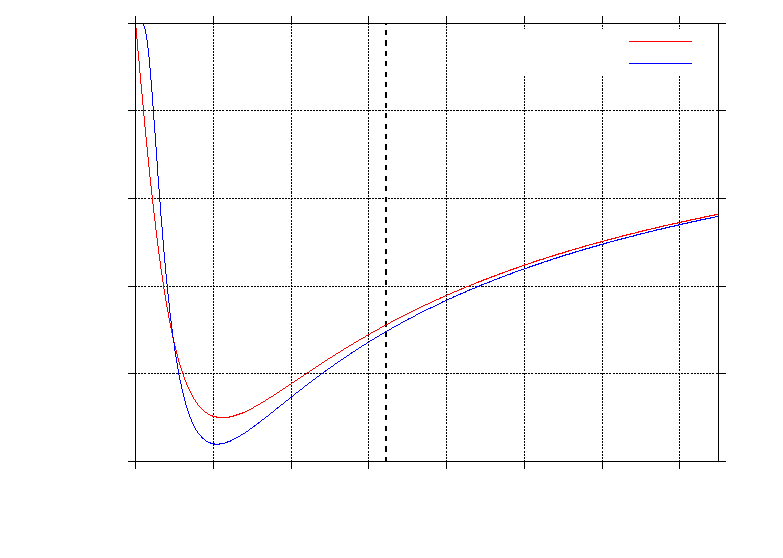
\includegraphics{Figures/twowires/InducedInteraction/InducedInteraction}}%
    \gplfronttext
  \end{picture}%
\endgroup
  
\caption{Solid lines: the effective interactions at the Fermi surface, $W^{ij}_{\text{ind}}(k_F,k_F)$, as a function of relative particle distance $n_F/n_B^{1/3}$. Red line: intrawire effective interaction, $W^{11}_{\text{ind}}(k_F,k_F)$. Blue line: interwire effective interaction, $W^{12}_{\text{ind}}(k_F,k_F)$. Dashed line: $v_F = c_0$. To the right hereof retardation effects are expected to kick in. Notice that the effective interactions have an extremal value. \\
Parameters: $k_Fd = 0.7$, $(n_Ba_B^3)^{1/3} = 0.01$, $(n_Ba_{BF}^3)^{1/3} = 0.1$, $m_B / m_F = 7/40$.}  
\label{fig.EffectiveInteraction.nBdepend}  
\end{center}    
\end{figure}

We notice that the \textit{inter}wire interaction becomes dominant around $n_Fn_B^{1/3} = 0.1$. This suggests that there will be a $p$- to $s$-wave phase transition around this value. Computing whether the intrawire effective interaction, $W^{11}_{\text{ind}}(k_F,k_F)$, or the interwire effective interaction, $W^{12}_{\text{ind}}(k_F,k_F)$, is dominant results in the dot-dashed curve in figure \ref{fig.twowirescrossovernBdepend}. 

\subsection{Phase diagram} \label{subsec.phasediagram}
Having considered the dependencies of both the interwire distance, $d$ and the Bose gas density, $n_B$, we can now plot the full phase diagram where both of these are varied. In this analysis we keep the Bose-Fermi gas parameter, $(n_Ba_{BF}^3)^{1/3}$, the Bose gas parameter, $(n_Ba_B^3)^{1/3}$ and the fermion density, $n_F$, constant. The relative particle distance, $n_F / n_B^{1/3}$ is varied by varying the Bose density, $n_B$.  

A direct and precise measure for the transition is the previously mentioned critical distance, $d_c$. In practice this is found in the following way. First we calculate the ground state energy $E_0(\Delta^{11}_k)$ in the case that there is only intrawire pairing, $\Delta^{11}_k$ present. This is independent of $d$ as described by the dashed curve in figure \ref{fig.2wiresE0ddepend}. Then we calculate the same, when only interwire pairing is present. For a constant $n_F/n_B^{1/3}$ we then iteratively find the value of $d = d_c$, where the ground state energies match: $E_0(\Delta^{12}_k, d_c) = E_0(\Delta^{11}_k)$. We then decrease $n_F/n_B^{1/3}$ by a small amount and repeat the process. The outcome of the analysis is shown as the black solid curve in figure \ref{fig.twowirescrossovernBdepend}. We notice that $d_c$ exhibits a maximal value and that it approaches a constant for large values of $n_F/n_B^{1/3}$. The dashed vertical line indicates where $v_F = c_0$. To the right of this line retardation effects are expected to kick in. 

The region with white background indicates the dominant \textit{intra}wire pairing regime. The grey area is correspondingly dominant \textit{inter}wire pairing. We can understand this result in the following way. First, consider a constant value of the relative particle distance, e.g. $n_F/n_B^{1/3} = 0.2$. When we decrease the interwire distance from say $k_Fd = 1$ we move along the dashed vertical grid line at $n_F/n_B^{1/3} = 0.2$. The system experiences the transition, when we cross the solid black line. This is as described in section \ref{sec.2wiresCrossover_energy}. Second, consider a constant value of the interwire distance, e.g. $k_Fd = 0.6$. When we increase $n_F/n_B^{1/3}$ we follow the horisontal grid line and the system again experiences the transition, when it crosses the solid black line. 

\begin{figure} 
\begin{center}  
% GNUPLOT: LaTeX picture with Postscript
\begingroup
  \makeatletter
  \providecommand\color[2][]{%
    \GenericError{(gnuplot) \space\space\space\@spaces}{%
      Package color not loaded in conjunction with
      terminal option `colourtext'%
    }{See the gnuplot documentation for explanation.%
    }{Either use 'blacktext' in gnuplot or load the package
      color.sty in LaTeX.}%
    \renewcommand\color[2][]{}%
  }%
  \providecommand\includegraphics[2][]{%
    \GenericError{(gnuplot) \space\space\space\@spaces}{%
      Package graphicx or graphics not loaded%
    }{See the gnuplot documentation for explanation.%
    }{The gnuplot epslatex terminal needs graphicx.sty or graphics.sty.}%
    \renewcommand\includegraphics[2][]{}%
  }%
  \providecommand\rotatebox[2]{#2}%
  \@ifundefined{ifGPcolor}{%
    \newif\ifGPcolor
    \GPcolorfalse
  }{}%
  \@ifundefined{ifGPblacktext}{%
    \newif\ifGPblacktext
    \GPblacktexttrue
  }{}%
  % define a \g@addto@macro without @ in the name:
  \let\gplgaddtomacro\g@addto@macro
  % define empty templates for all commands taking text:
  \gdef\gplbacktext{}%
  \gdef\gplfronttext{}%
  \makeatother
  \ifGPblacktext
    % no textcolor at all
    \def\colorrgb#1{}%
    \def\colorgray#1{}%
  \else
    % gray or color?
    \ifGPcolor
      \def\colorrgb#1{\color[rgb]{#1}}%
      \def\colorgray#1{\color[gray]{#1}}%
      \expandafter\def\csname LTw\endcsname{\color{white}}%
      \expandafter\def\csname LTb\endcsname{\color{black}}%
      \expandafter\def\csname LTa\endcsname{\color{black}}%
      \expandafter\def\csname LT0\endcsname{\color[rgb]{1,0,0}}%
      \expandafter\def\csname LT1\endcsname{\color[rgb]{0,1,0}}%
      \expandafter\def\csname LT2\endcsname{\color[rgb]{0,0,1}}%
      \expandafter\def\csname LT3\endcsname{\color[rgb]{1,0,1}}%
      \expandafter\def\csname LT4\endcsname{\color[rgb]{0,1,1}}%
      \expandafter\def\csname LT5\endcsname{\color[rgb]{1,1,0}}%
      \expandafter\def\csname LT6\endcsname{\color[rgb]{0,0,0}}%
      \expandafter\def\csname LT7\endcsname{\color[rgb]{1,0.3,0}}%
      \expandafter\def\csname LT8\endcsname{\color[rgb]{0.5,0.5,0.5}}%
    \else
      % gray
      \def\colorrgb#1{\color{black}}%
      \def\colorgray#1{\color[gray]{#1}}%
      \expandafter\def\csname LTw\endcsname{\color{white}}%
      \expandafter\def\csname LTb\endcsname{\color{black}}%
      \expandafter\def\csname LTa\endcsname{\color{black}}%
      \expandafter\def\csname LT0\endcsname{\color{black}}%
      \expandafter\def\csname LT1\endcsname{\color{black}}%
      \expandafter\def\csname LT2\endcsname{\color{black}}%
      \expandafter\def\csname LT3\endcsname{\color{black}}%
      \expandafter\def\csname LT4\endcsname{\color{black}}%
      \expandafter\def\csname LT5\endcsname{\color{black}}%
      \expandafter\def\csname LT6\endcsname{\color{black}}%
      \expandafter\def\csname LT7\endcsname{\color{black}}%
      \expandafter\def\csname LT8\endcsname{\color{black}}%
    \fi
  \fi
    \setlength{\unitlength}{0.0500bp}%
    \ifx\gptboxheight\undefined%
      \newlength{\gptboxheight}%
      \newlength{\gptboxwidth}%
      \newsavebox{\gptboxtext}%
    \fi%
    \setlength{\fboxrule}{0.5pt}%
    \setlength{\fboxsep}{1pt}%
\begin{picture}(7200.00,5040.00)%
    \gplgaddtomacro\gplbacktext{%
    }%
    \gplgaddtomacro\gplfronttext{%
      \csname LTb\endcsname%
      \put(176,2871){\rotatebox{-270}{\makebox(0,0){\strut{}$k_Fd_c$}}}%
      \put(3874,154){\makebox(0,0){\strut{}$n_F/n_B^{1/3}$}}%
      \csname LTb\endcsname%
      \put(814,767){\makebox(0,0)[r]{\strut{}$0$}}%
      \csname LTb\endcsname%
      \put(814,1469){\makebox(0,0)[r]{\strut{}$0.2$}}%
      \csname LTb\endcsname%
      \put(814,2170){\makebox(0,0)[r]{\strut{}$0.4$}}%
      \csname LTb\endcsname%
      \put(814,2872){\makebox(0,0)[r]{\strut{}$0.6$}}%
      \csname LTb\endcsname%
      \put(814,3573){\makebox(0,0)[r]{\strut{}$0.8$}}%
      \csname LTb\endcsname%
      \put(814,4275){\makebox(0,0)[r]{\strut{}$1$}}%
      \csname LTb\endcsname%
      \put(814,4976){\makebox(0,0)[r]{\strut{}$1.2$}}%
      \csname LTb\endcsname%
      \put(1009,484){\makebox(0,0){\strut{}$0$}}%
      \csname LTb\endcsname%
      \put(1773,484){\makebox(0,0){\strut{}$0.2$}}%
      \csname LTb\endcsname%
      \put(2537,484){\makebox(0,0){\strut{}$0.4$}}%
      \csname LTb\endcsname%
      \put(3301,484){\makebox(0,0){\strut{}$0.6$}}%
      \csname LTb\endcsname%
      \put(4066,484){\makebox(0,0){\strut{}$0.8$}}%
      \csname LTb\endcsname%
      \put(4830,484){\makebox(0,0){\strut{}$1$}}%
      \csname LTb\endcsname%
      \put(5594,484){\makebox(0,0){\strut{}$1.2$}}%
      \csname LTb\endcsname%
      \put(6358,484){\makebox(0,0){\strut{}$1.4$}}%
      \put(1850,3924){\makebox(0,0)[l]{\strut{}Intrawire pairing only}}%
      \put(4142,2521){\makebox(0,0)[l]{\strut{}Interwire pairing only}}%
    }%
    \gplbacktext
    \put(0,0){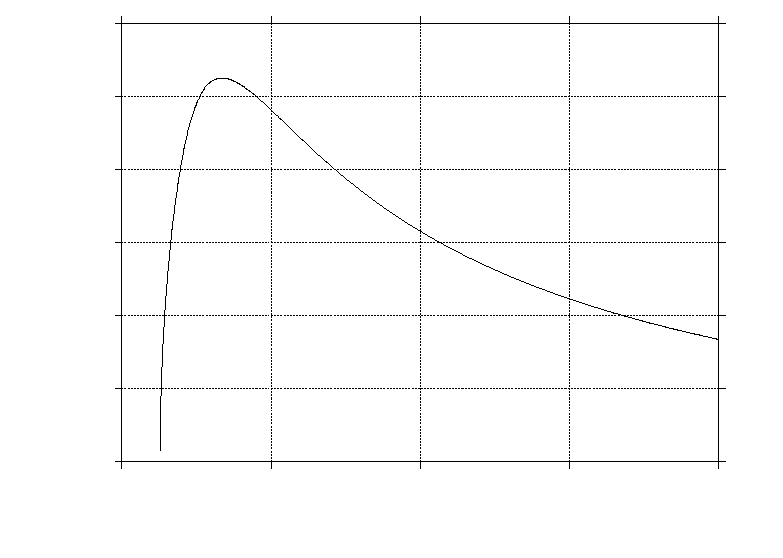
\includegraphics{Figures/twowires/Deltas3.1.3/nBdepend}}%
    \gplfronttext
  \end{picture}%
\endgroup
  
\caption{Phase diagram as a function of $d$ and $n_F/n_B^{1/3}$. Solid line: the critical distance $d_c$ plotted as a function of the relative particle distance $n_F/n_B^{1/3}$. White background: dominant intrawire pairing. Grey background: dominant interwire pairing. Dash-dotted line: the effective intra- and interwire interactions at the Fermi momentum are equal: $W^{12}_{\text{ind}}(k_F, k_F) = W^{11}_{\text{ind}}(k_F, k_F)$. We notice that the effective interactions give a qualitatively correct description. When we cross the solid line the system experiences the phase transition studied in section \ref{sec.2wiresCrossover_energy}. Dashed line: $v_F = c_0$. To the right hereof retardation effects are expected to kick in. Parameters: $(n_Ba_B^3)^{1/3} = 0.01$, $(n_Ba_{BF}^3)^{1/3} = 0.1$, $l_t = 0$, $m_B / m_F = 7/40$. }  
\label{fig.twowirescrossovernBdepend}  
\end{center}    
\end{figure}

In this way we explicitly see that instead of actually moving the wires we can control the transition by adjusting the relative interparticle distance, $n_F/n_B^{1/3}$, and in turn the coherence length; see equation \eqref{eq.RangefunctionofrBBnB}. We notice that the simple analysis based on the effective interactions at the Fermi momentum and the more elaborate but direct calculation of the critical distance $d_c$ are qualitatively similar. However, the dip in $d_c$ for high values of $n_F/n_B^{1/3}$ is more significant, than the simple analysis suggests. Further, there is a discrepancy in the position of the points at which the curves exhibit their maxima. This emphasizes the fact that although a lot of physical intuition can be build on the form and behaviour of the effective interactions, we have to be careful when used to argue for the response of the system.

\section{Physical discrepancies} \label{sec.physicaldiscrepancies}
The nontrivial result of the numerical analysis is that the energetically favourable choice for the interwire pairing is to break the $T^2 = -\mathbb{I}$ symmetry. This mean field result does however have an important physical discrepancy. Consider the gap equations for the double wire system, equation \eqref{eq.2wiresgapequations}. As we bring the wires closer together the intrawire pairing is not affected by the interwire induced interaction until an interwire pairing forms. This is absurd. The interwire interaction will of course alter the physical properties internally in each wire, also when the wires are far apart. 

The reason for this discrepancy is the following. When no mean field is present, the BCS mean field approximation is the same as neglecting the interaction all together. There is however a way to (partially) remedy this using the so-called Hartree-Fock self-energy. The self-energy is the energy shift a particle experiences due to its interaction with all the others. The self-energy for the fermions in the wires associated with the interwire interaction will therefore increase as the wires are brought closer together. In this way we can incorporate interaction effects without discarding the mean field approach all together. 

In section \ref{sec.meanfieldvalidity} we discussed the validity of the mean field approximation. The reader is referred thereto for a further discussion on the subject. 

